\documentclass[a4paper]{report}
\usepackage[utf8]{inputenc}
\usepackage[T1]{fontenc}
\usepackage[french]{babel}
\usepackage{geometry}
\geometry{hmargin=3.5cm,vmargin=3.5cm}
\usepackage{graphicx}
\usepackage{fancyhdr}
\usepackage{color}

\usepackage{listings}
\lstdefinestyle{styleXml}{
  basicstyle=\small,               % the size of the fonts that are used for the code
  breakatwhitespace=false,         % sets if automatic breaks should only happen at whitespace
  breaklines=true,                 % sets automatic line breaking
  frame=none,                      % adds a frame around the code
  keepspaces=true,                 % keeps spaces in text, useful for keeping indentation of code (possibly needs columns=flexible)
  keywordstyle=\color{blue},       % keyword style
  language=xml,                    % the language of the code
  morekeywords={Level,Cache,Architecture,...},            % if you want to add more keywords to the set
  numbers=none,                    % where to put the line-numbers; possible values are (none, left, right)
  rulecolor=\color{black},         % if not set, the frame-color may be changed on line-breaks within not-black text (e.g. comments (green here))
  stepnumber=2,                    % the step between two line-numbers. If it's 1, each line will be numbered
  stringstyle=\color{red},         % string literal style
  tabsize=4,                       % sets default tabsize to 2 spaces
  title=\lstname                   % show the filename of files included with \lstinputlisting; also try caption instead of title
}

\lstdefinestyle{styleMan}{
  basicstyle=\small,               % the size of the fonts that are used for the code
  breakatwhitespace=false,         % sets if automatic breaks should only happen at whitespace
  breaklines=true,                 % sets automatic line breaking
  frame=none,                      % adds a frame around the code
  keepspaces=true,                 % keeps spaces in text, useful for keeping indentation of code (possibly needs columns=flexible)
  keywordstyle=\textbf,            % keyword style
  language=tex,                    % the language of the code
  morekeywords={*,NAME,SYNOPSIS,DESCRIPTION,PARAMETERS,OPTIONS,AUTHORS,REPORTING,BUGS,COPYRIGHT,SEE,ALSO,EXAMPLE,FILE,DESCRPTION,...}
  numbers=none,                    % where to put the line-numbers; possible values are (none, left, right)
  rulecolor=\color{black},         % if not set, the frame-color may be changed on line-breaks within not-black text (e.g. comments (green here))
  tabsize=2,                       % sets default tabsize to 2 spaces
  title=\lstname                   % show the filename of files included with \lstinputlisting; also try caption instead of title
}
\lstset{language=xml, style=styleXml}
\lstset{language=tex, style=styleMan}
\usepackage{hyperref}
\hypersetup{colorlinks=true}

\pagestyle{fancy}

\lhead{Rapport}
\rhead{Simulateur de caches multi-c\oe ur}
\lfoot{ENSEIRB-MATMECA}
\rfoot{PFA 2013-2014}

\begin{document}

\thispagestyle{empty}

\vspace{\stretch{1}}
\hrule
\begin{flushleft}
\huge{Simulateur de caches sur\\architecture multi-c\oe ur :}\\
\end{flushleft}
\begin{flushright}
\Huge\textbf{Rapport}\\
\end{flushright}
\hrule

\vspace{\stretch{1}}
\noindent\textbf{Auteurs :}
\emph{DUBOIS Nicolas, GOUDET Pierre, HENG Nicolas, HONORAT Alexandre, MARAIT Gilles, PICHON Grégoire}\\
\\
\noindent\textbf{Client :}
\emph{M. BARTHOU Denis}\\
\\
\noindent\textbf{Responsable pédagogique :}
\emph{M. MORANDAT Floréal} 

\vspace{\stretch{1}}
\normalsize
\begin{center}
  Deuxième année, filière informatique\\
  Date : \today\\
  \textsc{Enseirb-Matmeca}
\end{center}


\newpage
\tableofcontents

\renewcommand{\labelitemi}{$\bullet$}

\newpage
\paragraph{}
Dans un ordinateur, les instructions du programme à exécuter ainsi que les données nécessaires
à son exécution sont stockées dans la mémoire. Le processeur exécute le programme en récupérant des informations dans celle-ci. De ce fait, la mémoire est un élément déterminant de performance car c'est elle qui est le facteur limitant du processeur : elle est son fournisseur.

\paragraph{}
Actuellement plusieurs types de mémoires sont présents dans un ordinateur, et les plus rapides sont les plus chères et également celles de plus petite taille.
Pour pallier au coût d'accès à l'espace mémoire, il existe ainsi une hiérarchie de la mémoire. Plus on s'éloigne du processeur, plus les mémoires sont grandes et peu chères, et en contrepartie, leur vitesse diminue. 

\paragraph{}
Dans le cadre de ce projet, nous nous intéressons à la mémoire cache. Dans la hiérarchie, elle se situe entre les registres du processeur et la mémoire RAM. Tout comme les registres, elle est interne au processeur.
Le point de départ du projet est que l'amélioration des performances d'un processeur, outre l'augmentation du nombre de c{\oe}urs ou de sa fréquence d'horloge peut également provenir de l'optimisation de sa mémoire cache. Le simulateur de caches \textsf{Cassis} a donc pour objectif d'étudier l'utilisation de la mémoire cache par un programme, afin de détecter une mauvaise utilisation des caches, ou de tester une nouvelle organisation des caches. Si les métriques obtenues par \textsf{Cassis} sont relativement peu utiles pour l'utilisateur lambda, elles peuvent néanmoins être très utiles pour la recherche, d'autant plus qu'il existe actuellement peu d'outils similaires.

\paragraph{}
Ce document s'adresse donc spécifiquement à des informaticiens désireux d'étudier le comportement de leurs programme, spécifiquement parallèles. Afin de comprendre comment \textsf{Cassis} fonctionne, il faut tout d'abord se familiariser avec la problématique qu'il est censé étudier : les caches. Tandis qu'une utilisation standard permettra de vérifier certains comportements de programmes et d'identifier plus précisément les causes de mauvaise utilisation des caches, l'utilisateur averti pourra configurer un certain nombre de paramètres afin de simuler des architectures actuellement inexistantes.

\newpage
\chapter{Généralités sur les caches}
Le but de cette partie est de résumer un certain nombre de techniques relatives à la gestion de la hiérarchie des caches. Nous commencerons par expliciter le comportement d'un cache en général, avant d'étudier les moyens mis en {\oe}uvre afin d'assurer la cohérence de l'ensemble des caches. Nous finirons par étudier les problèmes posés par la simulation des caches d'une architecture multi-c{\oe}urs, notamment le prefetching.

\subsection{Utilité des caches}

Jusqu'aux années 2000, la vitesse des processeurs a considérablement augmenté (loi de Moore) alors que le temps d'accès à la mémoire RAM (Random-Access Memory) est resté globalement le même. Pour permettre au processeur d'accèder plus rapidement à des éléments mémoire, des caches sont donc utilisés entre les processeurs et la RAM. Cela permet de hiérarchiser la mémoire, avec des éléments dont le temps d'accès est différent. Cette organisation hiérarchique de la mémoire présente plusieurs objectifs : \\
\begin{itemize}
\item permettre de contenir un nombre conséquent de données ;
\item être organisée de manière à être rapide ;
\item ne pas coûter trop cher.\\ 
\end{itemize}

Les caches permettent de stocker la mémoire utilisée récemment par le processeur, en se basant sur deux concepts: la localité spatiale et la localité temporelle. La localité temporelle stipule qu'une cellule mémoire accédée récemment sera très probablement utilisée dans un futur proche. La localité spatiale est l'idée que si l'on accède à une cellule mémoire $X$, la cellule mémoire $X+1$ a de grandes chances d'être utilisée. \\

Les mémoires de haut niveau -- les plus proches du processeur sont notées L1 -- sont généralement de petite taille. Leur coût est conséquent mais leur accès est très rapide. Il existe plusieurs niveaux de caches, $3$ dans la plupart des architectures récentes. Les L1 sont très rapides mais peuvent contenir peu de données (de l'ordre de la dizaine de Ko) alors que le L3 est plus lent mais contient beaucoup de données (de l'ordre du Mo). On peut résumer comme par la figure \ref{img:hierarchy} une hiérarchie mémoire classique.\\

\begin{figure}[!h]
\begin{center}
   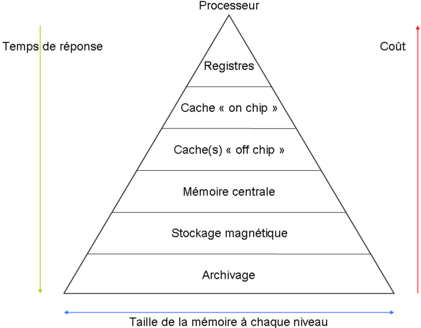
\includegraphics[scale=0.75]{images/hierarchy.png}
   \caption{\label{img:hierarchy} Hiérachie mémoire}
\end{center}
\end{figure}

%==> Préciser source de l'image + légende\\

De cette manière, quand le processeur utilise une donnée qui est dans le cache, il fait un \textit{hit} : il n'a pas besoin de la charger à partir de la mémoire principale. Lorsque la donnée dont il a besoin n'est pas présente dans le cache, il fait un \textit{miss} et le coût d'accès à la donnée est beaucoup plus important. \\

Les données mémoire vont être lues via des \textit{load} et écrites via des \textit{store}. Lorsqu'une donnée est modifiée, il est nécessaire de propager les modifications jusqu'à la mémoire principale (c'est donc un \textit{store}), afin de garantir la cohérence du système. Une politique basique, le \textit{write-through}, serait de réécrire directement en mémoire après toute modification. Dans la suite de ce document, nous considérerons uniquement la politique \textit{write-back}, qui permet de retarder la réecriture tant que la donnée n'est pas lue pas une autre entité que celle qui l'a modifiée.

\section{Principes généraux d'un cache}
Cette section entend préciser le fonctionnement général d'un cache : comment il est possible d'y ajouter une donnée, quelle est la correspondance entre les blocs de la mémoire principale et les lignes de cache ou encore comment une donnée peut être evincée d'un cache. \\

Un cache possède un ensemble de sets contenant chacun un ensemble de lignes. Le nombre de lignes par set est appelé l'associativité du cache. Au chargement d'une donnée, elle est insérée dans une ligne vide du set correspondant à sa plage d'adresse. Les données qui suivent (dans la mémoire supérieure) la donnée voulue sont aussi recopiées afin de remplir totalement la ligne -- généralement de $32$ ou $64$ octets -- et exploiter le principe de localité spatiale (footnote ?).

\subsection{\'Etiquettes}
Pour pouvoir retrouver une donnée dans le cache, une table d'étiquettes est tenue à jour. Concrètement, une adresse mémoire est séparée en trois champs comme sur la figure suivante : \\

\begin{figure}[!h]
\begin{center}
   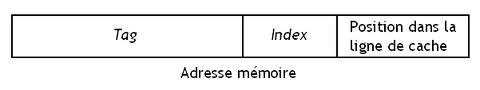
\includegraphics[scale=0.50]{images/etiquette.jpeg}
   \caption{\label{img:etiquette} Adresse mémoire}
\end{center}
\end{figure}

%==> Préciser source de l'image\\

Le tag est stocké dans la table des étiquettes, il servira a identifier les différents blocs mémoires pouvant être au même endroit dans un cache. L'index correspond au numéro de set dans lequel se trouve la ligne de cache. Pour finir l'offset correspond au bloc dans la ligne de cache.

\subsection{Fonction de correspondance}
Un cache de taille $n$ contient un ensemble $p$ de lignes de taille $m$, tel que $n = p \times m$. Afin de placer et récupérer une donnée dans le cache, une fonction de correspondance avec la mémoire est nécessaire. Il existe trois cas de figure. Pour la suite, nous prendrons : \\
\begin{itemize}
\item $i$ le numéro de set du cache
\item $j$ le numéro du bloc mémoire
\item $s$ le nombre de sets du cache
\item $k$ l'associativité du cache 
\end{itemize}

\subsubsection{Direct associative}
Un cache est en correspondance directe si à chaque bloc mémoire est associé une unique ligne du cache. Le nombre de sets, $s$, du cache est alors égal à son nombre de lignes, $p$. Lorsqu'un bloc mémoire $j$ est ajouté dans le cache, la ligne correpondante est chargée à la ligne $i = j\ modulo\ s$. Avec ce type de cache, il est facile d'ajouter ou de retrouver une données. Cependant, si plusieurs blocs mémoires correpondant à la même ligne de cache sont fréquemment utilisés, il faudra sans cesse supprimer et ajouter des données dans le cache.

\subsubsection{Fully associative}
Un cache est en correspondance associative si chaque bloc mémoire peut être mis dans n'importe quelle ligne du cache. Il n'y a alors qu'un seul set. L'inconvénient précédent n'est plus existant, cependant il devient beaucoup plus compliqué de rechercher une donnée dans le cache. L'ensemble des étiquettes doit en effet être parcouru.

\subsubsection{$k$-ways associative}
Les deux cas présentés précedemment présentent des inconvénients. Généralement, un cache profite des avantages des deux visions en faisant un compromis. Dans le cas de la correspondance associative par ensemble, chaque set possède un nombre $k$ de lignes tel que $p=k \times s$. La fonction de correspondance est telle que $i = j\ modulo\ s$. De cette manière, un bloc mémoire peut se trouver dans un ensemble de $k$ lignes. Il est donc possible d'avoir plusieurs blocs mémoires correspondant au même ensemble et l'algorithme de recherche est plus efficace que dans le cas de la correspondance associative.

\begin{figure}[!h]
\begin{center}
   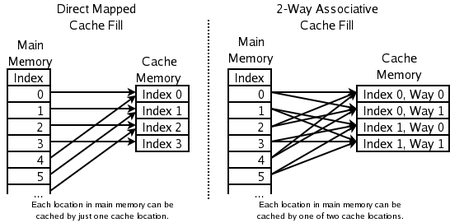
\includegraphics[scale=0.60]{images/associative.png}
   \caption{\label{img:associative} Fonction de correspondance}
\end{center}
\end{figure}

%==> Préciser source de l'image\\

\subsection{Politiques de remplacement}
\label{remplacement}
 Lorsque l'on souhaite ajouter une ligne dans un set plein, il faut au préalable évincer une ligne de ce set. Pour cela, il existe différentes méthodes :

\paragraph{FIFO.} La première solution consiste à supprimer la ligne la plus ancienne du cache. Cela correspond à la formule: ``First In, First Out''.

\paragraph{LFU.} Une autre solution consiste à supprimer la ligne qui a été le moins utilisée: ``Least Frequently Used''. Pour cela, chaque ligne de cache possède un compteur qui sera incrémenté à chaque utilisation de la ligne. 

\paragraph{LRU.} La dernière solution, généralement utilisée, consiste à favoriser le principe de localité temporelle en supprimant la ligne du set qui a la plus ancienne date d'utilisation: ``Least Recently Used''.

\section{Gestion de la cohérence}
Dans les systèmes actuels, un processeur n'est plus composé d'un unique c{\oe}ur, mais de plusieurs. Chaque c{\oe}ur possède généralement deux caches qui lui sont propres : le L1i pour stocker les instructions et le L1d pour stocker les données. Les caches de niveau supérieur sont quant  eux partagés par un nombre variable d'autres caches (et c{\oe}urs). Alors que les interactions entre ces deux premiers caches sont minimes -- il est difficile de mélanger instructions et données --, la cohérence entre les autres est en revanche un problème de taille.

\subsection{Présentation du problème}
Les caches sont utilisés à chaque \textit{load}/\textit{store}. S'il est possible que plusieurs caches possèdent la même donnée et la lisent en même temps, il est primordial qu'une donnée ne puisse pas être modifiée simultanément dans deux caches. Pour cela, des techniques hardware sont mises en place afin de définir qui a la priorité si plusieurs c{\oe}urs veulent modifier une même donnée. \\

\begin{figure}[H]
\begin{center}
   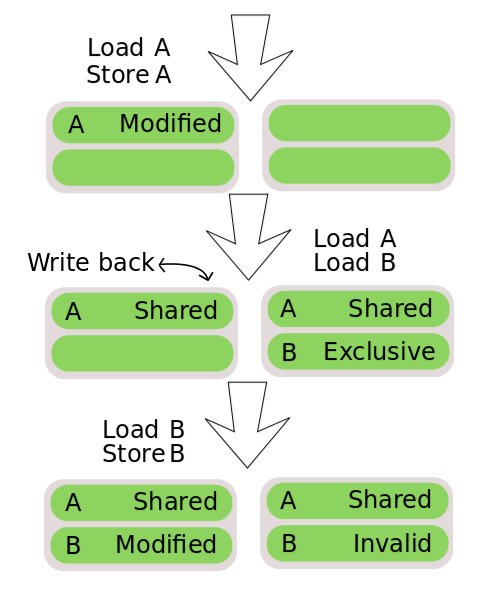
\includegraphics[scale=0.35]{images/learn_mesi_2.png}
   \caption{\label{img:mesi} Utilité d'un protocole de cohérence}
\end{center}
\end{figure}

Par ailleurs, un protocole de cohérence est mis en {\oe}uvre à chaque \textit{load}/\textit{store} afin que les différents caches soient informés des modifications les concernant et que la consistance du système soit assurée. Ce protocole est propre à un niveau de cache. Dans un cas classique, il y aura un protocole de cohérence entre les L1 et entre les L2.

\subsection{Protocoles de cohérence}
\label{coherence}
 Nous étudierons uniquement le protocole de type MSI et ses dérivés : MESI, MOSI et MOESI. Chaque ligne de cache possède un état qui permet de gérer la cohérence. Les différents états sont: \\
\begin{itemize}
\item M: Une ligne est dans l'état modifié si c'est la seule copie valide dans l'ensemble des caches du niveau. Dans ce cas, si la ligne est evincée du cache, elle doit être recopiée en mémoire, via un write back. \\
\item S: Une ligne est dans l'état partagé (\textit{shared}) si elle est valide et qu'elle n'a pas été modifiée. Dans ce cas, plusieurs caches peuvent possèder la ligne. \\
\item I: L'état invalide est utilisé pour une ligne qui n'est pas valide. Le contenu de la ligne n'étant pas viable, il ne faut pas l'utiliser. \\
\item E: Une ligne est dite exclusive si elle est, dans le niveau, la seule copie valide. Une ligne dans cet état n'a pas été modifiée et les données de la ligne sont identiques à celles de la mémoire principale. \\
\item O: L'état \textit{owned} est utilisé pour un cache qui possède une donnée invalide dans la mémoire principale. Plusieurs caches peuvent possèder la même donnée, ils seront alors dans l'état S. \\
\end{itemize}

L'état M est utilisé lorsque la donnée a été modifiée par un c{\oe}ur. Il existe deux cas de propagation des modifications. Dans le choix de la politique \textit{write-through}, la donnée est directement recopiée dans la mémoire principale pour éviter de futurs problèmes de cohérence. Dans le cas de la politique \textit{write-back}, la donnée est modifiée uniquement dans le cache. Les autres caches et la mémoire principale peuvent savoir que la donnée a été modifiée, en revanche ils n'ont pas la dernière copie valide. Ils peuvent l'obtenir lors des \textit{Write-Back}: lorsque la donnée est evincée du cache ou lorsqu'elle est demandée à un plus haut niveau pour des soucis de cohérence.\\

Le protocole de cohérence le plus utilisé est MESI. Voici certaines caractéristiques de ce protocole : \\
\begin{itemize}
\item Lorsqu'un cache charge une donnée, il demande si un autre cache possède la donnée. Si un cache possède la donnée dans l'état M, alors ce cache fait un Write-Back et invalide sa donnée. Si un autre cache possède la donnée en état E, la donnée passe dans l'état S pour les deux caches. Si plusieurs (ou un seul) caches possèdent la donnée dans l'état S, la donnée est ajoutée dans l'état S.
\item Si un cache possède une donnée dans l'état M ou E et fait un nouveau \textit{store} sur la ligne de cache, son état devient M et aucune information n'est transmise aux autres caches.
\item Si un cache fait un \textit{store} sur une donnée qui est dans l'état S, la même donnée est invalidée dans les autres caches du même niveau. \\
\end{itemize}

Le protocole est souvent représenté sous la forme d'un automate, dont les états possibles sont ceux des données : \\

\begin{figure}[!h]
\begin{center}
   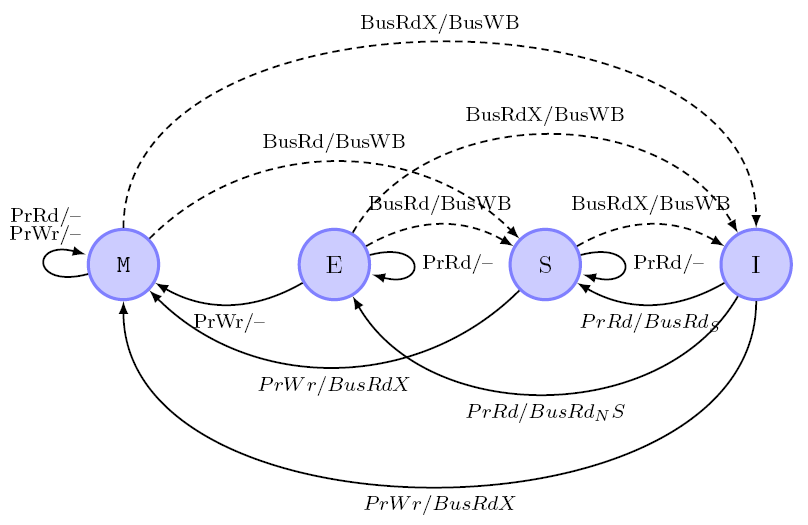
\includegraphics[scale=0.45]{images/mesi.png}
   \caption{\label{img:mesi} Automate du protocole MESI}
\end{center}
\end{figure}

%==> Préciser source de l'image + légende\\

Pour l'état O, la différence est que les interactions avec la mémoire principale sont moins importantes. En effet, lorsqu'un cache qui n'a pas la donnée fait un \textit{load}, le cache possédant la donnée dans l'état O peut lui donner sans faire de \textit{write-Back}. Cela permet de garder plus longtemps la donnée modifiée.

%\newpage
\section{Fonctionnement global}
La cohérence expliquée jusqu'à présent correspondait à celle d'un niveau de caches. Mais il peut arriver d'autres problèmes de gestion des données entre ces différents niveaux car les niveaux de caches peuvent être inclusifs, exclusifs ou non-inclusifs. Par ailleurs, les particularités du snooping, qui consiste à demander via un bus une donnée aux autres caches du même niveau, seront aussi explicitées. \\

Le cas inclusif est plutôt orienté \textsf{Intel} alors que le cas exclusif est plutôt mis en place par \textsf{AMD}. De son côté \textsf{ARM} oscille entre les deux solutions proposées.

\label{inclusivite}
\subsection{Caches inclusifs}
Le fonctionnement d'un cache inclusif est relativement simple. En cas de \textit{hit}, la donnée est propagée au cache (ou au processeur) qui a préalablement demandé la donnée. En cas de \textit{miss}, une demande de donnée est effectuée au niveau du dessus. La donnée est ensuite propagée à la mémoire d'en dessous. Dans le cas d'une hiérarchie avec uniquement des caches inclusifs, les messages utilisés pour demander/donner les données se font uniquement de façon verticale dans la hiérarchie. Il y a parallèlement, des messages destinés à garantir la consistance du système qui sont gérés différemment et qui influent sur la totalité de la hiérarchie. Voici un résumé des messages envoyés dans le cas d'une demande de donnée, en ne tenant pas compte de la gestion de la cohérence : \\

\begin{figure}[!h]
\begin{center}
   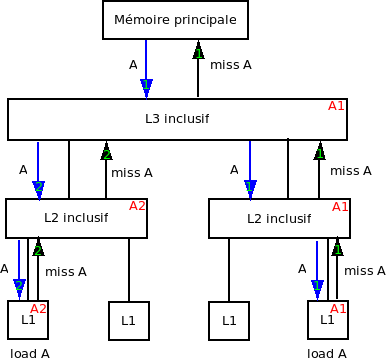
\includegraphics[scale=0.7]{images/inclusifs.png}
   \caption{\label{img:inclusifs} Caches de niveau 2 et 3 inclusifs}
\end{center}
\end{figure}

%==> Préciser source de l'image + légende\\

\subsection{Caches exclusifs}
Cependant, le fait qu'un cache soit inclusif pose un problème : les données sont dupliquées dans la hiérarchie. De ce fait, la taille réellement utilisable de l'ensemble des caches est en fait inférieure à la taille théorique. Les caches exclusifs ont justement pour principal objectif de limiter cette duplication des données. Par exemple, si un L2 est exclusif, les L1 en dessous ne pourront pas contenir une donnée déjà présente dans le L2, et inversement. Concrètement, il y a quatre cas de figure : \\

%==>un joli schéma\\
\begin{itemize}
\item Si un L1 fait un \textit{hit}, il transmet la donnée au c{\oe}ur associé
\item Si un L2 fait un \textit{hit}, il donne la donnée au L1 qui l'a demandé puis la supprime.
\item Si un L1 fait un \textit{miss}, il effectue une demande de donnée au L2 associé. Il gardera la donnée une fois qu'elle lui sera transmise.
\item Si un L2 fait un \textit{miss}, il effectue une demande de donnée au L3 associé, ou directement à la mémoire principale si il n'y a pas de L3. Une fois que la donnée lui sera transmise, il la propagera au L1 sans la conserver. \\
\end{itemize}

Il en va de même pour les interactions entre les L2 et les L3, voire d'autres niveaux dans le cas d'une architecture plus grande. Par ailleurs, lorsque le dernier niveau fait un \textit{miss}, il faut parcourir l'ensemble de la hiérarchie avant de rechercher directement la donnée dans la mémoire principale. Ce phénomène explique à lui seul le fait que la gestion de la recherche et de la cohérence soit plus délicat que dans le cas d'une hiérachie avec le dernier niveau inclusif.

\subsection{Caches non-inclusifs}
Il existe un autre cas de figure, qui peut être considéré comme une variante du cas exclusif. Lorsqu'un L1 demande une donnée et que le L2 ne l'a pas, il se contentera de propager la donnée sans la conserver en mémoire. Cependant, si il avait préalablement la donnée, il la propagera au L1 sans pour autant la supprimer. Ce cas de figure peut être utilisé pour un L2 avec un L3 inclusif. De cette manière, la hiérarchie permet en moyenne de stocker plus de blocs mémoires sans pour autant compliquer la gestion de la cohérence. \\

Un autre cas de figure est un cache non-inclusif qui fonctionne avec plus de souplesse qu'un cache inclusif. Les données sont toujours laissées au passage, par contre l'inclusivité n'est pas formelle: il peut perdurer dans un L1 une donnée qui a été ejectée d'un L2 par exemple.

\subsection{Ajout du snooping}
\label{snooping}
 Il est possible que les caches d'un même niveau soient reliés ensemble par un bus. La méthode de recherche sur ce bus est alors appelée snooping. Prenons l'exemple d'une hiérarchie à trois niveaux où les L2 seraient reliés par un bus. Lorsqu'un L1 fait un \textit{miss}, il demande au L2 associé de lui fournir la donnée. En cas de nouveau \textit{miss}, la demande est envoyée en broadcast sur le bus afin de récupérer la donnée sans passer par le L3. Si aucun cache ne possède la donnée, la demande est alors transmise au L3.

\newpage
\section{Comportements spéciaux}
Les politiques de remplacement, de cohérence et les différents types de caches offrent un ensemble de modularités dans la gestion d'une hiérarchie de caches. Cependant, d'autres possibilités existent afin d'améliorer les performances de l'ensemble.

\subsection{Utilisation d'un \textit{victim cache}}
Généralement, des caches à $k$ voies associatifs sont utilisés, car la fonction de recherche d'une donnée est peu coûteuse et plusieurs blocs mémoire correspondant à un même set peuvent être stocké dans un cache. Dans la plupart des cas, le nombre de voies varie entre $2$ et $12$. \\

Dans certains cas, il est possible que le nombre de voies ne soit pas suffisant car un ensemble de blocs mémoire correspondant au même set est très utilisé. Cela est notamment vrai pour les L1 qui possèdent généralement peu de voies. Pour pallier ce problème et limiter les échanges de données entre les L1 et les L2, il est possible d'utiliser un buffer pour stocker les victimes d'éviction. Ce buffer est de petite taille, par exemple $8$ fois la taille d'une ligne de cache. De cette manière, lorsqu'un donnée est supprimée du L1, elle est placée dans le buffer correspondant. Lorsque le L1 fait un \textit{miss}, il commence par regarder dans le buffer (le coût est alors faible). Les données arrivant dans le L2 sont alors celles evincées du buffer.

\subsection{Suivi des données}
 Il existe différentes manières de localiser les données dans une hiérarchie mémoire -- il ne s'agit pas ici de la recherche au sein d'un cache, cela est géré par la table d'étiquettes, mais bien entre les caches. Deux cas fréquents se posent, ils sont réglés la plupart du temps par un \textit{tracking} : dans quels caches se trouvent les données.

\subsubsection{Supprimer les données}
Lorsqu'un cache L1 utilise une donnée qu'il possède déjà dans son cache, les flags utilisés par les politiques de remplacement sont mis à jour afin de supprimer les bonnes données lorsqu'un set sera plein. Cependant, les caches de plus haut niveau (L2, L3) ne sont pas mis au courant que la donnée a été utilisée et ils ne changent donc pas les flags de remplacement. Ainsi, lorsque le L2 aura un set plein, il se peut qu'il supprime une donnée très utilisée dans un L1. \\

Dans le cas d'un cache inclusif, il faut donc, à la suppression d'une donnée, invalider la donnée dans les caches en dessous afin de conserver le caractère inclusif. Pour limiter ce problème, les L2 et les L3 peuvent suivre les données, c'est-à-dire posséder une table indiquant quels caches de niveau plus bas ont également la donnée. De cette manière, les politiques de remplacement peuvent être adaptées en définissant des priorités: par exemple, éviter de supprimer les données qui sont contenues dans beaucoup de caches.

\subsubsection{Savoir qui a les données}
Dans le cas d'un cache de dernier niveau et exclusif, s'il se produit un \textit{miss}, il faut parcourir l'ensemble de la hiérarchie avant d'évenetuellement faire appel à la mémoire principale. Cela pose des problèmes, tant au niveau de la recherche des données que de la gestion de la consistance du système. Pour pallier ce problème, le cache de dernier niveau peut être lié à un table d'étiquettes, permettant de savoir quelles sont les données contenues dans chaque cache. Cela évite d'avoir à parcourir l'ensemble de la hiérarchie mais il y a un coût en terme de mémoire. Cependant, ce coup est faible (les données ne sont pas stockées) et bien inférieur au coût mémoire de la duplication dans le cache d'un cache de dernier niveau inclusif.

\newpage
\chapter{Presentation du simulateur de caches : \emph{Cassis}}
\textsf{Cassis} est un simulateur de caches sur architecture multi-c\oe ur développé dans le cadre d'un PFA -- Projet au Fil de l'Année -- à l'\textsc{Enseirb-Matmeca}, sur une idée proposée par Denis BARTHOU pour le compte de l'\textsf{INRIA}. L'\textsf{INRIA} est un institut publique de recherche français en informatique et automatismes ; et bien que ce projet soit réalisé dans un cadre scolaire, l'objectif est de le rendre utilisable par les équipes de recherche des thématiques associées aux caches et au parallèlisme.

\section{Cadre du simulateur}

\paragraph{}
Un simulateur est un programme qui va reproduire le fonctionnement d'un système afin de pouvoir en étudier certaines caractéristiques de manière moins contraignante que sur le système réel. Dans le cas du programme \textsf{Cassis}, c'est l'utilisation des caches par un programme donné qui est simulée.

\subsection{Origine du projet}

\paragraph{}
La mémoire est de nos jours l'un des principaux facteurs de ralentissement des programmes. Une mauvaise gestion de la mémoire peut être désastreuse au niveau des performances, et pourtant, il n'existe pas de moyen efficace et précis de connaître l'utilisation de la mémoire au niveau des caches. Le but de \textsf{Cassis} est donc d'étudier l'utilisation précise des caches par un programme, afin d'aider l'utilisateur à tester les performances du programme, ainsi que les analyser pour les améliorer.

\paragraph{}
Le besoin d'un tel simulateur est avant tout dû au manque d'informations sur les caches. Deux phénomènes se produisent du côté des constructeurs de processeurs. D'une part ils doivent les optimiser afin d'être concurrents, et il devient alors difficile pour eux de fournir des fonctionnalités dédiées aux développeurs afin d'améliorer leur code, par exemple une meilleure connaissance des politiques utilisées. D'autre part il n'est pas dans leur intérêt de révéler le fonctionnement de leurs produits, pour des raisons économiques évidentes. Par exemple, le \emph{prefetching} permet de charger des lignes de caches en avance en fonction des accès mémoires courants du programme et cette fonctionnalité n'est pas implémentée dans le simulateur car son fonctionnement n'est pas totalement divulgué.

\paragraph{}
L'intérêt d'un tel simulateur est donc de pouvoir tester des programmes en produisant certaines statistiques, mais aussi de pouvoir tester l'exécution sur des architectures qui n'existent pas afin de connaître la pertinence d'une nouvelle politique de cohérence par exemple. Seuls les caches de données sont simulés, le but étant d'essayer d'optimiser la mémoire d'un programme. Le chargement du code du programme est fait par le processeur sans intervention de l'utilisateur.

\subsection{Outils à disposition de l'utilisateur}

Le simulateur s'appuie sur des outils préexistants, pour la génération des traces et de l'architecture. Les outils listés ci-dessous sont ceux utilisés par l'équipe de projet. Si d'autres outils offrent des fonctionnalités similaires, ils peuvent être utilisés en remplacement tant que les fichiers d'entrée du programme sont dans le bon format.

\paragraph{HWLOC} est un logiciel qui permet de récupérer l'architecture des caches d'une machine. Il permet de générer un fichier xml que nous enrichissons. La paramétrisation de l'architecture des caches ne prend pas en compte les caches d'instructions, mais seulement les caches de données. L'utilisation de ce fichier est détaillé dans la section \ref{param_xml}.

\paragraph{MAQAO} (Modular Assembly Quality Analyzer and Optimizer) est un outil d'analyse et d'optimisation de programmes. Une seule fonctionnalité de \textsf{MAQAO} est utilisée, celle qui permet d'instrumenter un programme binaire afin de récupérer les instructions réalisées pendant l'exécution. Le paramétrage de \textsf{MAQAO} est effectué grâce à un fichier lua pour générer des traces de la forme voulue.

\paragraph{}
L'utilisateur peut aussi vouloir comparer les résultats de la simulation. Bien qu'il n'existe par actuellement de tel simulateur pour faire la comparaison, il existe des compteurs hardware -- par exemple \textsf{PAPI} -- qui permettent de connaître certaines statistiques sur les caches. Les limites du simulateur seront donc étudiées, afin de valider son bon fonctionnement par rapport au comportement attendu.

\section{Déroulement de la simulation}

\paragraph{}
La simulation consiste à rejouer un certain nombre d'instructions, et à comptabiliser certaines métriques à destination de l'utilisateur. Comme il s'agit d'une simulation, tout ne se passe pas exactement comme dans le cas réel. Il est donc nécessaire d'expliciter les similitudes comme les différences afin que l'utilisateur ne soit pas surpris à la fois par les résultats et par les méthodes de calculs si son objectif est de modifier le code.

\paragraph{}
Dans le cadre de la simulation, seules les références aux données sont stockées en mémoire, c'est-à-dire l'ensemble des étiquettes qui permettent d'identifier les différentes données. Pour une ligne de cache de taille $64$ octets par exemple, seule la première case est réellement stockée en mémoire, les $56$ autres octets correspondant aux données sont inutiles pour réaliser les statistiques.

\subsection{Traitement d'une instruction : load/store}

\paragraph{}
La simulation, même d'un programme parallèle, est une séquence d'instructions effectuant des modifications (lecture ou écriture) sur les caches. Les deux premières possibilités pour une instruction sont une lecture de donnée ou une écriture. Une fois le type d'instruction connu, il faut la faire correspondre au c{\oe}ur sur lequel elle a été effectuée. Si la donnée est déjà présente dans le cache de plus bas niveau (L1), alors il s'agit d'un \emph{hit}. Sinon, il faut rechercher la donnée dans la hiérarchie. A noter que pour des raisons d'efficacité, la simulation ajoute la donnée au moment même où l'on traite le cache: on prévoit qu'elle sera bientôt fournie par un cache de niveau supérieur en cas de \emph{miss}.

\paragraph{}
L'idée de l'algorithme est donc la suivante: on applique l'instruction courante au L1 correspondant, et si la donnée n'est pas présente, on remonte au niveau d'au dessus. Les protocoles de cohérence étant relatifs à un niveau donné, ils sont appliqués dès que possible afin d'éviter d'avoir à monter puis à redescendre dans la hiérarchie pour des questions de complexité. Cette idée de prévision permet généralement de gagner du temps mais pose certains problèmes qui seront explicités.

\paragraph{}
Un algorithme pour le traitement général d'une instruction est le suivant: 
\begin{enumerate}
  \item{il s'agit d'un \emph{load} ou d'un \emph{store}}
  \item{la donnée est présente dans le cache ou non
      \begin{enumerate}
      \item{si non, l'ajouter et faire :}
      \item{appel de la procédure de suppression en cas de cache plein}
      \item{mettre à jour les états de cohérence des différents caches du niveau concernés par la même donnée}
      \item{chercher la donnée dans la hiérarchie avec du \emph{snooping} ou un \emph{directory manager}}
      \item{revenir au point 2 s'il faut chercher la donnée dans un cache de plus haut niveau}
  \end{enumerate}}
  \item{mettre à jour les statistiques de remplacement sachant qu'une ligne a été accédée}
  \item{dans le cas d'un \emph{store}, propager l'action de modification dans tous les caches de niveaux supérieurs}
\end{enumerate}

\paragraph{}
Dans le code du simulateur, le traitement d'une instruction différe dans le cas d'un \emph{load} ou d'un \emph{store}. En effet les deux versions se distinguent par la dernière étape, où dans le cas d'un \emph{store}, les caches parents doivent être prévenus de la modification même en cas de \emph{hit}. Si par exemple, en cas de \emph{hit} lors d'un \emph{store} d'une donnée A dans un L1, le L2 doit être informé afin de pouvoir invalider la même donnée dans les autres L2. Cependant, si la lecture du programme apparaît comme une vraie modification des données (comme pour la politique \emph{write-through}), les statistiques sont bien réalisées de manière à suivre le cas du \emph{write-back}, où une modification dans un cache de bas niveau provoque une réécriture dans les caches de plus haut niveau le plus tard possible afin de limiter le coût de ces échanges entre les caches.

\paragraph{}
Le paragraphe précédent fait apparaître quelques uns des problèmes issus de la manière prédictive de voir les choses. Les problèmes fondamentaux sont la recherche d'une donnée dans la hiérarchie, l'ajout d'une ligne dans un cache, et la conservation des propriétés des caches inclusifs et exclusifs.

\subsection{Rapatriement prédictif d'une ligne}

\paragraph{}
Le fait de supposer qu'il est possible d'ajouter une donnée avant même de l'avoir trouvée dans la hiérarchie ne change rien au niveau des statistiques produites, mais impose de prendre soin à certaines étapes du traitement d'une instruction. En cas de \emph{miss}, trois traitements peuvent être réalisés, selon l'architecture fournie en entrée du programme. Une première solution consiste à rechercher les données par \emph{snooping}, c'est-à-dire parmis les caches du même niveau partageant le même parent. Cette étape doit être réalisée avant la mise à jour des états de cohérence. Par exemple en cas de \emph{store} sur une donnée, avec la politique de cohérence MESI, les autres caches vont devoir invalider leur copie locale de la même donnée pour garantir la cohérence. D'où l'obligation de réaliser le protocole de \emph{snooping} avant d'éventuelles invalidations.

\paragraph{}
\label{directorymanager}
Une seconde solution consiste à utiliser un \emph{directory manager}, afin de rechercher les données dans les caches en dessous (impossible pour un L1). Dans l'implémentation choisie, le traitement par \emph{directory manager} implique de réellement parcourir l'ensemble des caches ayant pour parent le cache courant. Dans le cas réel, une table comportant la partie étiquette des lignes de caches est tenue à jour grâce à un \emph{directory manager}. Cependant, vu la complexité des messages à envoyer pour garantir la consistance de la table, le choix du parcours de tous les caches a été réalisé.

\paragraph{}
Si la donnée n'a pas été trouvée via le \emph{snooping} ou grâce à un \emph{directory manager}, une demande est effectuée au cache de plus haut niveau qui effectue une autre recherche jusqu'à éventuellement joindre la mémoire principale.

\paragraph{}
La particularité du rapatriement prédictif des données est à prendre en compte dans l'écriture des politiques de cohérence. En effet certaines politiques se basent sur la présence ou non de la même ligne dans le niveau du cache demandant la donnée, voir à ce sujet les conditions de transitions d'automates dans la partie \ref{aut}. Il faut alors être conscient que la donnée est déjà dans le niveau lorsque les voisins sont prévenus.

\subsection{Problème d'ajout de ligne dans un cache plein}

\paragraph{}
L'ajout d'une donnée dans un cache est également un problème compliqué. Il faut commencer par identifier dans quel bloc la donnée va se retrouver, puis demander à la politique de remplacement un emplacement dans ce bloc pour mettre la nouvelle donnée. Si le bloc n'était pas plein, l'ajout d'une ligne dans un cache se résume à trouver le bloc et ajouter la donnée.

\paragraph{}
Cependant, si le cache est plein, une ligne à evincer est choisie. Il faut ensuite rapatrier cette ligne dans le cache de niveau supérieur, si elle n'y était pas déjà présente et faire un \emph{write-back} si la ligne supprimée avait été modifiée. Si la donnée n'était pas présente dans le cache de niveau supérieur, il faut l'y ajouter. Une subtilité relative au traitement prédictif de la recherche d'une donnée est alors à prendre en compte. En effet, si un L1 ajoute une donnée $A$ et qu'il doit pour cela supprimer la donnée $B$, il va falloir ajouter cette donnée dans le L2 correspondant. Or si ce L2 est plein, il peut évincer la donnée $A$. Le traitement étant prédictif, ce n'est pas la situation qui se produirait dans la réalité. Pour pallier à ce problème, une donnée à ne surtout pas supprimer à été ajoutée en paramètre des fonctions relatives au remplacement.


\subsection{Gestion des différents types de cache}
\paragraph{}
\textsf{Cassis} permet de gérer différents types de caches: inclusif, exclusif, non-inclusif orienté inclusif et non-inclusif orienté exclusif. Si la gestion des caches non-inclusifs est assez souple (on ne connaît pas précisément les choix faits par les constructeurs), la gestion des caches inclusifs et exclusifs s'attache à assurer que le type des caches est bien respecté.

\paragraph{}
Pour un cache inclusif, le cas problématique est la suppression d'une donnée. Il faut en effet assurer que les caches de plus bas niveau ayant pour parent le cache inclusif ne conservent pas la donnée. La solution mise en {\oe}uvre consiste à invalider dans toute la hiérarchie en dessous de ce cache. Une gestion plus subtile est possible par une utilisation des \emph{directory manager}. Avant de supprimer une donnée, les caches en dessous sont consultés afin de connaître les données qu'ils possèdent. De cette manière, des priorités sont calculées pour la suppression des données, afin d'éviter d'avoir à invalider d'autres caches.

\paragraph{}
Ce problème est crucial au sens où il est très fréquemment rencontré. En effet, les politiques de remplacement peuvent être différentes entre les niveaux et dans une certaine mesure incohérentes. Si un cache L2 possède un remplacement de type FIFO alors que les L1 associés ont un remplacement de type LRU, les flags de remplacement vont faire que le L2 aura tendance à vouloir supprimer des données qui peuvent avoir été récemment utilisées dans les L1.

\paragraph{}
Pour un cache exclusif, il faut assurer qu'une donnée qu'il possède ne se trouve pas ailleurs dans ses fils et réciproquement. Pour cela, lorsqu'un cache exclusif fait un \emph{hit}, il supprime la donnée correspondante car elle a été demandée par un de ses fils.

\section{Données simulées : analyse des statistiques}

Différentes statistiques sont relevées par le simulateur, les principales sont les \emph{misses}, les \emph{hits} et les \emph{write-backs}. Dans l'exemple ci dessous, on peut observer une sortie standard de \textsf{Cassis}:
\begin{lstlisting}
L3  basics   (misses:   6, hits:   0, writes_back:   0)
L2  basics   (misses:   6, hits:   0, writes_back:   0)
L1  basics   (misses:   4, hits:  44, writes_back:   1)
L2  basics   (misses:   7, hits:   2, writes_back:   0)
L1  basics   (misses:   6, hits:  42, writes_back:   2)
L2  basics   (misses:   0, hits:   0, writes_back:   0)
L1  basics   (misses:   0, hits:   0, writes_back:   0)
L2  basics   (misses:   6, hits:   3, writes_back:   0)
L1  basics   (misses:   0, hits:   0, writes_back:   0)
\end{lstlisting}


Voici par ailleurs, une sortie possible de \textsf{HWLOC} correspondant à la même architecture: \\
\begin{figure}[H]
\begin{center}
   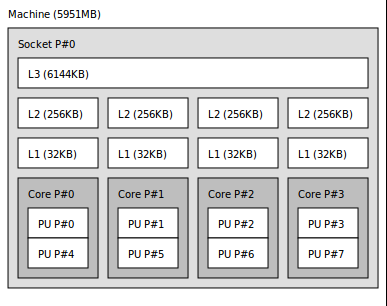
\includegraphics[width=0.7\textwidth]{images/lstopo.png}
   \caption{\label{img:archi} Sortie possible de \textsf{HWLOC}}
\end{center}
\end{figure}

Par rapport à la sortie du simulateur, le premier L2 qui apparaît correspond au $Core \ P\#0$.

Il est également possible d'avoir plus de statistiques, voici le schéma maximal pour un seul cache:
\begin{lstlisting}
L1  basics     (misses:      8, hits:        40, writes_back:   4)
    evinctions (coherence:   4, capacity:    0, cache_types:    0)
    misses     (snooping:    3, above:       5, below:          0)
    broadcasts (coherence:   10, snooping:   8)
\end{lstlisting}


Ces statistiques ont été choisies afin que l'utilisateur puisse constater certains problèmes particuliers. Par exemple, un nombre trop élevé de \emph{write-backs} et/ou de \emph{coherence evinctions} révèle que les c\oe urs modifient les mêmes données et que la manière de paralléliser le code n'est donc pas efficace. \\

L'affichage des statistiques est configurable en ligne de commande, avec l'option \texttt{-v i}, pour $i$ allant de $1$ à $4$, selon le nombre de lignes de statistiques à afficher. La première ligne correspond aux statistiques de base, qui ont déjà été vues. \\

Par rapport aux evictions de données, trois cas se présentent:
\begin{itemize}
\item coherence: ce cas se produit lorsqu'une donnée est invalidée dans un cache à cause d'une écriture dans un autre cache,
\item capacity: c'est le cas ``classique `` d'éviction: la taille du cache est trop faible pour contenir beaucoup de données,
\item cache\char`_types: ce cas se produit lorsqu'un cache exclusif donne une donnée: il doit l'invalider pour garantir l'exclusivité; ou encore lorsqu'un cache inclusif invalide une donnée: il doit également l'invalider dans les niveaux en dessous afin de conserver le caractère inclusif. \\ 
\end{itemize}

En cas de \emph{Miss}, trois solutions sont possibles pour trouver les données dans la hiérarchie:
\begin{itemize}
\item snooping: la donnée est obtenue via du \emph{snooping} avec un cache de même niveau,
\item above: la donnée est obtenue en remontant dans la hiérarchie,
\item below: la donnée est obtenu en parcourant la hiérarchie vers les niveaux inférieurs. Dans le cas étudié, cette situation ne peut se présenter qu'avec l'utilisation de \emph{directory manager}. \\
\end{itemize}

Pour finir, deux types de \emph{broadcast} font partie des statistiques:
\begin{itemize}
\item coherence: cette statistique permet de comptabiliser les échanges de messages nécessaires aux politiques de cohérence, pour que les lignes des caches soient dans les bons états,
\item \emph{snooping}: quand un cache fait une demande pour récupérer une donnée via le snooping. \\
\end{itemize}


Mais les statistiques ne sont pas les seuls paramètres d'analyse, la sélection des données à analyser à aussi un rôle important. Le simulateur permet de suivre les statistiques d'une ou plusieurs instructions données, et ainsi de déterminer quelles instructions causent des ralentissements à l'exécution, i.e. un trop grand nombre de \emph{misses}.

\subsection{\'Etapes de validation}
\begin{frame}
  \begin{block}{Pr\'esentation}
    \begin{itemize}
      \item Tests unitaires
      \item Validation durant le programme
      \item Comparaison avec des outils existants
      \item Benchmarks
    \end{itemize}
  \end{block}
  \begin{block}{Premiers outils de v\'erification}
    \begin{itemize}
      \item Validation des politiques basiques
      \item Validation du comportement inclusif
      \item Utilisation de \textsf{PAPI}
    \end{itemize}
  \end{block}
\end{frame}

\begin{frame}{Benchmarks basiques}
\begin{figure}[H]
   \begin{minipage}[l]{.46\textwidth}
     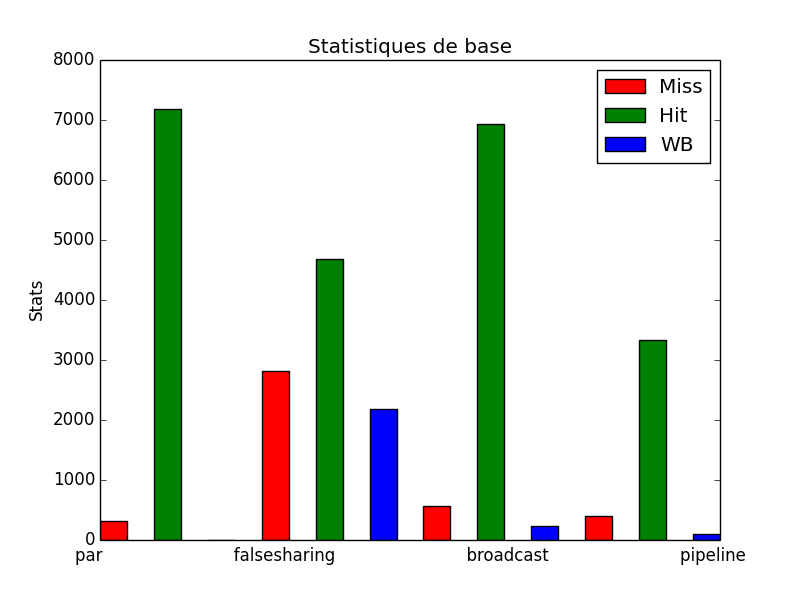
\includegraphics[scale=0.22]{images/stats_L1.png}
   \end{minipage} \hfill
   \begin{minipage}[r]{.46\textwidth}
     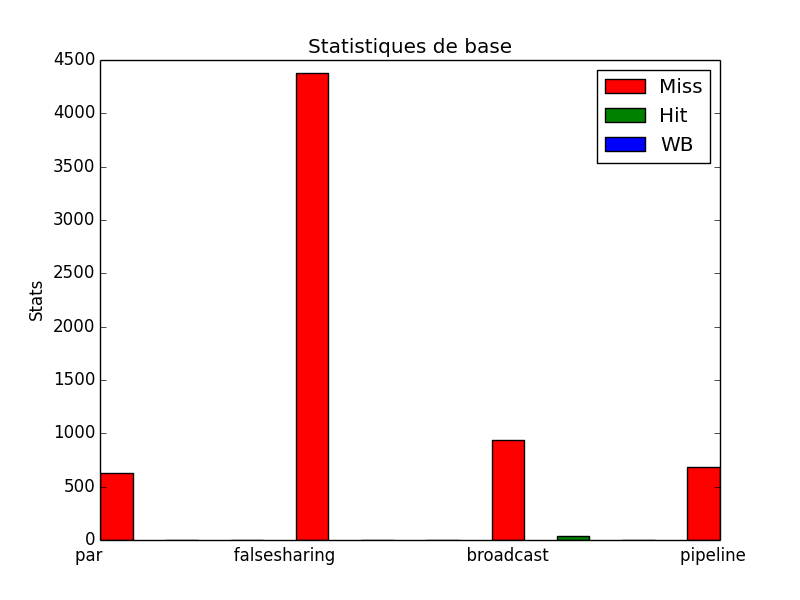
\includegraphics[scale=0.22]{images/stats_L2.png}
   \end{minipage}
\end{figure}

\begin{figure}[t!]
  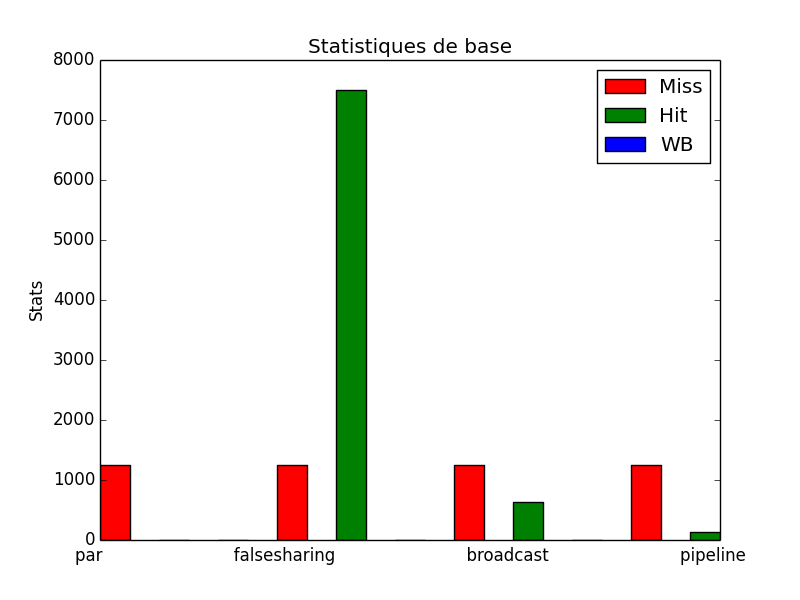
\includegraphics[scale=0.22]{images/stats_L3.png}
\end{figure}
\end{frame}

\begin{frame}{Benchmarks avanc\'es}
\begin{figure}[H]
   \begin{minipage}[l]{.46\textwidth}
     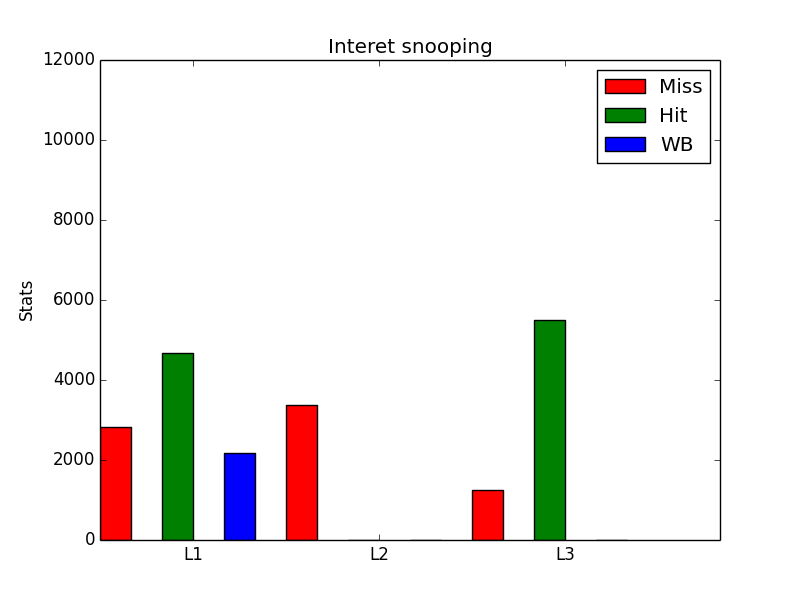
\includegraphics[scale=0.22]{images/stats_falsesharing_snooping.png}
   \end{minipage} \hfill
   \begin{minipage}[r]{.46\textwidth}
     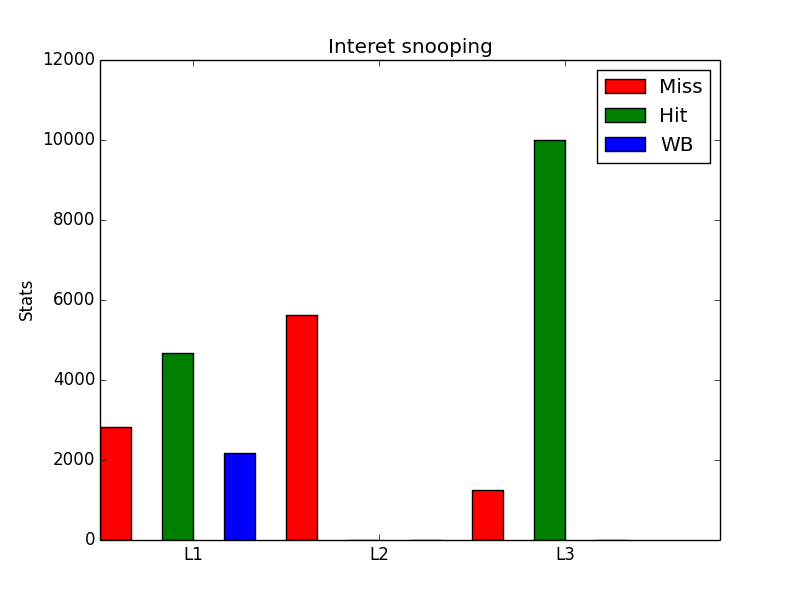
\includegraphics[scale=0.22]{images/stats_falsesharing_no_snooping.png}
   \end{minipage}
\end{figure}
  \begin{block}{Autres benchmarks}
    \begin{itemize}
      \item \emph{Directory manager}
      \item Politiques de coh\'erence MSI vs MESI
      \item Scalabilit\'e
    \end{itemize}
  \end{block}
\end{frame}

\subsection{Limites \`a  propos de la simulation des caches}
\begin{frame}
  \begin{block}{Probl\`emes li\'es aux architectures multi-c{\oe}ur}
    \begin{itemize}
      \item \textsf{prefetching}
      \item synchronisations
      \item changements de contextes 
    \end{itemize}
  \end{block}
  \begin{block}{Limites de \textsf{Cassis}}
    \begin{itemize}
      \item bande passante non mod\'elis\'ee
      \item \textsf{Directory manager} basiquement mod\'elis\'es
      \item statistiques non calibr\'ees avec des benchmarks classiques
      \item utilisation de m\'etriques non usuelles
    \end{itemize}
  \end{block}
\end{frame}


\section*{Conclusion}
\begin{frame}
  \begin{block}{Objectifs atteints}
    \begin{itemize}
      \item Cahier des charges respect\'e
      \item Param\'etrisation compl\`ete
    \end{itemize}
  \end{block}

  \begin{block}{\'Evolution possible}
    \begin{itemize}
      \item Complage avec un simulateur \textsf{on-line}?
      \item Utilisation de benchmarks pour calibrer les r\'esultats?
    \end{itemize}
  \end{block}
\end{frame}

\section{Format d'une trace}
Actuellement, le simulateur utilise en entrées des traces fournies par \textsf{MAQAO}. Bien qu'il soit envisageable d'utiliser un autre format de trace respectant la vision interne au simulateur, le suivi des données reste propre au format de sortie de \textsf{MAQAO}.

\subsection{Présentation du format}
Deux étapes sont nécessaires à la création des traces par \textsf{MAQAO}. La première consiste à instrumenter un fichier source, écrit en \textsf{C} et en \textsf{OpenMP}. Chaque instruction possède un numéro, un type, et notamment une référence à la ligne du code source. A noter que cette référence peut parfois être erronée, à cause des optimisations du compilateur. Pour limiter ce problème, il est préférable de compiler avec les options \texttt{-g -O0}. \\

Voici un exemple de sortie de cette première étape: \\
\begin{framed}
\begin{verbatim}
  1 - Intrumented LOAD (MOV)@400c61 SRC@27 par._omp_fn.3
  2 - Intrumented LOAD (MOV)@400c6e SRC@27 par._omp_fn.3
  3 - Intrumented LOAD (MOV)@400c72 SRC@27 par._omp_fn.3
  4 - Intrumented STORE (MOV)@400c82 SRC@27 par._omp_fn.3
  5 - Intrumented LOAD (ADD)@400c85 SRC@27 par._omp_fn.3
  6 - Intrumented LOAD (CMP)@400c89 SRC@27 par._omp_fn.3
  7 - Intrumented LOAD (MOV)@400ce9 SRC@31 par._omp_fn.4
  8 - Intrumented LOAD (MOV)@400cf6 SRC@31 par._omp_fn.4
  9 - Intrumented LOAD (MOV)@400cfa SRC@31 par._omp_fn.4
\end{verbatim}
\end{framed}

La seconde étape consiste à executer l'executable produit. Il en résulte un ensemble d'instructions (\emph{load} ou \emph{store}). Chaque ligne présente le type d'instruction, l'adresse virtuelle sur laquelle est réalisée l'instruction, le numéro du threads et l'instruction correspondante. L'utilisation d'adresse virtuelle impose de prendre des précautions avec l'utilisation des traces. En créant les traces deux fois à partir d'un même programme, le résultat obtenu n'est pas le même.\\

Voici un exemple de la seconde sortie: \\
\begin{framed}
\begin{verbatim}
LOAD 7fff71d376b0 1 11
LOAD 1660c18 1 12
STORE 1660c18 1 13
LOAD 7f0b333d0e1c 1 14
LOAD 7f0b333d0e1c 1 15
LOAD 7f0b333d0e1c 1 6
LOAD 7f0b333d0e08 1 7
LOAD 7fff71d376b0 1 8
LOAD 7f0b333d0e1c 1 9
LOAD 7fff71d371b0 3 11
LOAD 1670c18 3 12
STORE 1670c18 3 13
\end{verbatim}
\end{framed}

A la fin de cette seconde étape, un script \textsf{awk} est utilisé afin de créer une trace par thread. L'ensemble des traces constituera une des entrées de \textsf{Cassis}.

\subsection{Suivi de données spéciales}
Avec le format de traces décrit précédemment, il est possible de suivre certaines données en particulier. Le premier choix consiste à suivre une plage d'adresses virtuelles, cela est rendu possible avec l'option \texttt{-b @a:@b} qui permet de suivre les données comprises entre l'adresse de $a$ et l'adresse de $b$. \\

Il est également possible de suivre des instructions avec l'option \texttt{-i i1:i1} pour par exemple suivre uniquement les instructions $i1$ et $i2$. Le résultat obtenu en utilisant les deux options citées est l'intersection des données suivies. \\

Ce suivi d'instructions permet d'autres opportunités. Un script permet de recenser les instructions relatives à chaque ligne du code source, il est donc possible de connaître les statistiques pour une ligne donnée. Cette idée offre des perspectives, notamment par rapport à l'annotation du code source, pour par exemple indiquer les lignes qui posent des problèmes du point de vue des caches.



\newpage
\chapter{Paramétrisation du simulateur}
Un simulateur présente l'intérêt de se dégager de certaines contraintes imposées aux expériences sur des systèmes réels. La simulation ne serait donc que peu utile s'il existait trop de contraintes. La forte paramétrisation du simulateur \textsf{Cassis} était donc un objectif impératif, introduit dès la phase de spécification des besoins. Il convient d'avoir la possibilité de simuler des programmes sur des architectures et des politiques de cohérence et d'entrelacement descriptibles facilement. Des langages spécifiques ont été utilisés pour chacun des aspects, afin soit de permettre une modification rapide des paramètres de simulation sans recompilation, soit de permettre une modification dans un language adapté au problème.

\section{Paramétrisation de l'architecture}

L'architecture à simuler peut être générée à partir de l'architecture réelle de l'utilisateur au moyen d'un fichier XML créé par le logiciel \emph{HWLOC}. Cependant l'utilisateur peut utiliser un fichier de paramétrisation spécifique à notre simulateur qui lui permet d'accéder à l'intégralité des paramètres d'architecture pris en compte.

\subsection{Entrée XML HWLOC}

\emph{HWLOC} est un logiciel libre sous liscence BSD-2. Il permet de générer un fichier XML qui décrit l'architecture de la machine utilisée (commande \verb?lstopo --of xml?). Il décrit notamment la structure arborescente des caches, et donne des informations essentielles pour chaque cache, comme sa taille, la taille de ses lignes et son associativité. 

\paragraph{}
Si l'utilisateur choisit un tel fichier en entrée comme décrivant son architecture, ce dernier sera parsé en un fichier de configuration de l'architecture personnalisé, comme décrit dans la section \ref{config}. Les paramètres non fournis par le fichier généré par \emph{HWLOC} prendront des valeurs par défaut, proches de celles des architectures \emph{intel} moderne. Notons que notre simulateur ne prend pas en compte les caches de niveau 1 dédiés aux instructions (L1i), qui sont décrits par \emph{HWLOC} mais ne seront pas présent dans le fichier personnalié.

\subsection{Fichier de configuration personnalisé}
\label{config}
Le fichier de configuration de l'architecture dédié à notre simulateur comprend tous les paramètres d'achitecture utilisables. Une fois généré à partir d'un fichier \emph{HWLOC}, il est possible de l'utiliser directement en entrée du simulateur, après avoir été modifié à la convenance de l'utilisateur.

\paragraph{}
Il s'agit d'un fichier XML qui contient 3 balises :
\begin{itemize}
  \item \textbf{Architecture} : donne le nom de l'architecture et du modèle de microprocesseur utilisé, ainsi que le nombre de niveaux de cache.
  \item \textbf{Level} : décrit un niveau de cache. Pour chaque profondeur, le protocole de cohérence, le type d'inclusivité, la présence ou non de \textit{snooping} et d'un \textit{directory manager}.
  \item \textbf{Cache} : décrit l'arborescence des caches. Pour chaque cache, sa profondeur, sa taille, la taille de ses lignes, son associtivité et son protocole de remplacement.
\end{itemize}

\subsubsection{Paramètres de la balise Architecture}

\begin{itemize}
  \item \textbf{name} : nom de l'architecture (ex : \textit{x86\_64})
  \item \textbf{CPU\_name} : modèle du microprocesseur
  \item \textbf{number\_levels} : nombre de niveaux de cache
\end{itemize}

\subsubsection{Paramètres de la balise Level}

\begin{itemize}
  \item \textbf{depth} : la profondeur du niveau. La valeur doit être cohérente avec le nombre de niveaux de l'architecture.
  \item \textbf{coherence\_protocol} : \verb?MESI? ou \verb?MSI?
  \item \textbf{type} : \verb?inclusive?, \verb?exclusive?, \verb?niio? (Non Inclusive, Inclusive Oriented) ou \verb?nieo? (Non Inclusive, Exclusive Oriented)
  \item \textbf{snooping} : \verb?true? ou \verb?false?
  \item \textbf{directory\_manager} : \verb?true? ou \verb?false?
\end{itemize}

\subsubsection{Paramètres de la balise Cache}
Ces balises doivent former l'arborescence des caches.

\begin{itemize}
  \item \textbf{depth} : la profondeur du cache.
  \item \textbf{cache\_size} : taille du cache (en octets)
  \item \textbf{cache\_linesize} : taille d'une ligne de cache (en octets)
  \item \textbf{cache\_associativity} : associativité du cache
  \item \textbf{remplacement\_protocol} : \verb?FIFO?, \verb?LRU? ou \verb?LFU?
\end{itemize}

\subsubsection{Exemple de fichier}

%TODO : mettre un exemple de fichier à jour


\begin{frame}
 \frametitle{Nécessité de l'entrelacement}
 Architecture multi-coeur => Exécution parallèle\\
 \'Etat des caches dépendant de l'orde d'exécution
 \begin{figure}
   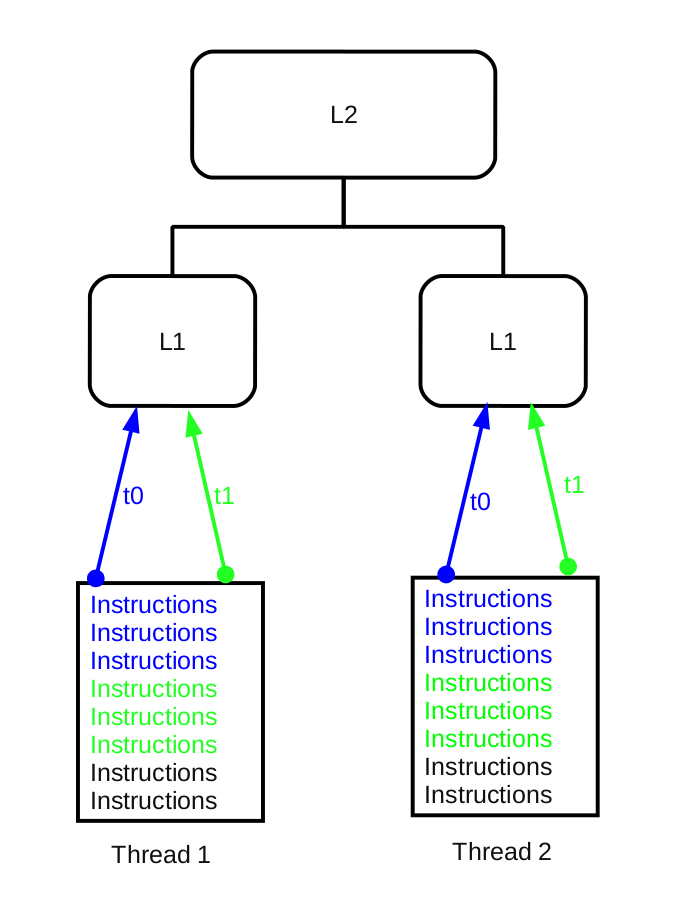
\includegraphics[scale=0.3]{images/schema_entrelacement.png}
 \end{figure}
\end{frame}

\begin{frame}
 \frametitle{Entrelacement dans CASSIS}
 Entrelacement bloc par bloc:
 \begin{figure}
   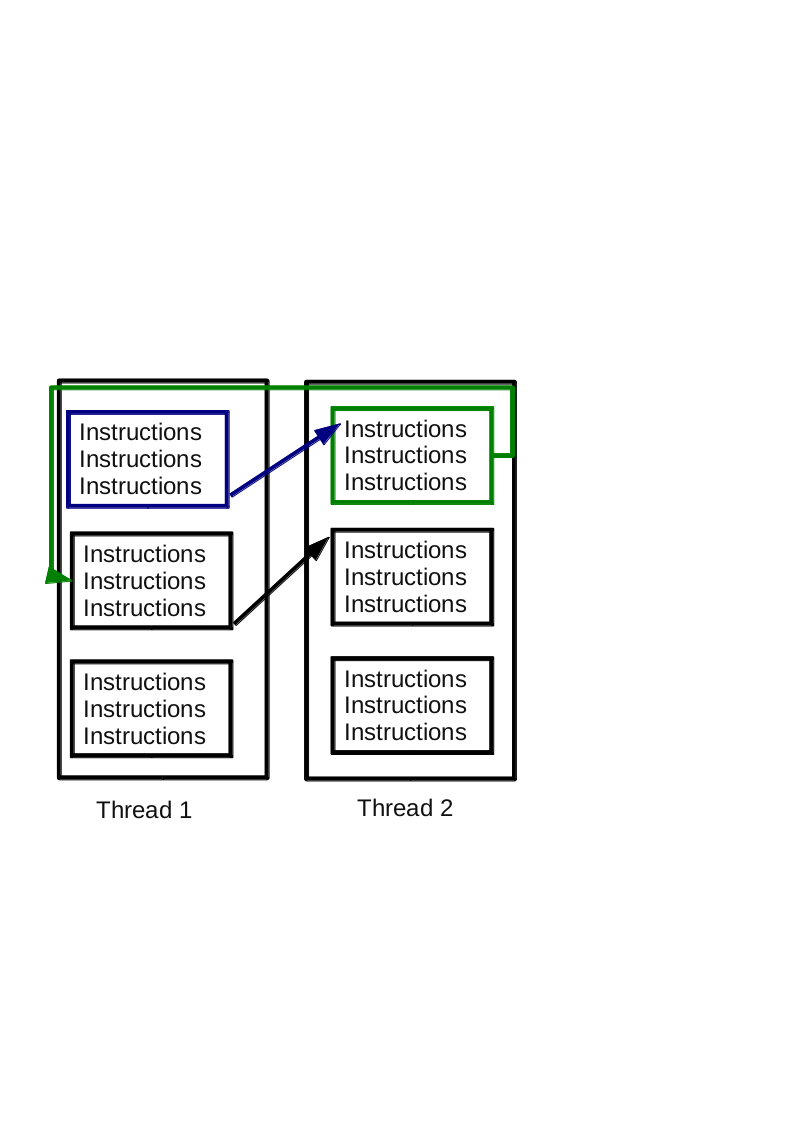
\includegraphics[scale=0.4]{images/schema_lua.png}
 \end{figure}
\end{frame}

\section{Gestion des politiques de coherence}

Les politiques de cohérence pré-implémentées sont MSI, MESI, MOESI, MESIF et MOSI. Elles sont nécessaires pour décrire l'état d'une ligne dans un cache et se représentent facilement par des automates dont les états sont ceux de la ligne, et les transitions sont des actions effectuées sur la ligne. Il est possible de rajouter d'autres politiques comme expliqué dans le tutoriel de la partie \ref{tuto_aut}, la section ci-dessous a pour vocation uniquement de préciser la paramétrisation des politiques déjà définies, sans évoquer la syntaxe à utiliser.

\subsection{Actions réalisées par une politique de cohérence}
\label{actions}

\paragraph{}
Une politique de cohérence est utilisée afin de garantir la cohérence des données dans tous les caches d'un même niveau : c'est-à-dire éviter qu'un cache ne possède une donnée qui n'est pas à jour car modifiée par un autre cache. L'objectif des constructeurs est donc de limiter les invalidations de lignes ou les messages de cohérence (voire l'envoi de la ligne) entre les caches, en cas de modification d'une ligne par un cache tiers. 

\paragraph{}
Dans le cas de \textsf{Cassis}, les politiques de cohérence s'occupent donc simplement de modifier le nouvel état de la ligne en cas d'action sur celle-ci. Les actions (qui sont donc les transitions des automates) peuvent être une lecture, une écriture ou une suppression, par le cache-même ou par un des caches du même niveau. Certaines statistiques dépendent aussi de ces actions. Ainsi les \verb!COHERENCE_EVINCTION!, \verb!COHERENCE_BROADCAST! et les \verb!WRITE_BACK! sont comptabilisées par les politiques de cohérence, respectivement dans le cas d'une invalidation de la ligne pour cause de modification dans un autre cache, pour l'envoi d'un message ou d'une donnée aux autres caches et enfin pour l'écriture de la donnée dans le cache parent. 

\subsection{Utilisation de SMC}

\paragraph{}
Afin de décrire facilement ces automates, l'utilsateur dispose d'un unique fichier à modifier qui contient toutes les desciptions de politiques. Celui-ci est rédigé grâce à un DSL -- Domain Specific Language -- nommé \textsf{SMC}, pour State Machine Compiler. Le fichier concerné est \verb!coherence.sm! situé au niveau des sources dans le dossier \verb!state-machine!. Il nécessite pour générer le code \texttt{C} associé d'une version standard de \texttt{Java}.

\paragraph{}
Ce DSL permet de définir plusieurs automates, dont les transitions sont les fonctions à appeler pour modifier leur état. \textsf{SMC} tel qu'utilisé dans le simulateur permet de réaliser plusieurs opérations : décrire les états de l'automate, décrire les transitions (entre états d'un même automate ou non), appliquer des conditions aux transitions, et enfin effectuer des actions spécifiques lors de l'appel d'une transition.

\paragraph{}
Certaines subtilités peuvent toutefois sembler complexe pour l'utilisateur : par exemple le nommage des fonctions possibles à l'intérieur du fichier de description. Les règles typographiques des transitions, et les possibilités d'action sont restreintes, voir pour cela la partie \ref{tuto_aut}.

\subsection{\'Ecriture d'une politique}

\paragraph{}
La première phase de l'écriture d'une politique est de pouvoir l'initialiser. En effet l'automate de départ n'est qu'un automate de départ vers les politiques : la première transition appelée correspond au choix de la politique, et va placer l'automate dans l'état I (\emph{invalid}) de la politique voulue. Il faut donc ajouter la transition dans l'automate de départ du fichier, automate nommé \texttt{Init} et ne comportant qu'un seul état mais autant de transitions que de politiques différentes.

\paragraph{}
Chaque politique doit donc contenir au moins l'état I ; et pour chaque état qu'elle définit elle peut ajouter des transitions, éventuellement conditionnelles. Les actions réalisées lors d'une transition doivent contenir à la fois les statistiques si nécessaires et à la fois la modification de l'état dans la structure contenant l'automate. En effet il n'a pas été possible de récupérer l'état courant de l'automate nécessaire à certaines fonctions. Cet état doit donc être sauvegardé dans la structure d'une ligne, en plus de la structure même de l'automate. Il s'agit d'une duplication d'information nécessaire au fonctionnement général du simulateur, et dû à des problèmes d'interfaçage entre le \texttt{C} et \textsf{SMC}.

\paragraph{}
\`A la fin de chaque description de politique se trouve un certain de nombre de transitions par défaut. Si elles sont appelées sur un état ne les définissant pas, elles bouclent dessus. Cela sert à factoriser les transitions n'effectuant aucune action sur un état.

\subsection{\'Eléments paramétrisables}

\paragraph{}
Les éléments dits paramétrisables de ce fichier, sont ceux qui ne nécessitent pas d'intervention dans d'autres fichiers du code source. Il n'est ainsi pas possible de rajouter de nouveau type de transition ou de nouvel automate, car ceux-ci ne seraient pas appelées par le programme principal. Sont donc modifiables : \\
\begin{itemize}
\item{les noms des états et des automates, il est aussi possible d'enlever ou d'ajouter d'autres états,}
\item{les actions des transitions, i.e. la modification de l'état tel que visible par le simulateur et l'incrémentation d'une statistique déjà existante,}
\item{les transition conditionnelles (en rajouter ou supprimer mais uniquement en utilisant les fonctions de tests préexistantes),}
\item{les transitions par défaut et actions associées (en rajouter ou supprimer).}
\end{itemize}

\paragraph{}
Deux fonctions sont disponibles pour les tests des transitions conditionnelles, il s'agit pour l'une de savoir si une ligne est marquée comme \emph{dirty} ou non, et pour l'autre de savoir si une ligne est présente ailleurs dans le niveau, avec possibilité de chercher une ligne dans un état spécifique. Attention, si l'état en paramètre est I, alors ce sont toutes les lignes valides qui sont recherchées. Il n'est donc pas possible de savoir si une ligne est dans l'état I ailleurs dans le niveau.





\newpage
\chapter*{Conclusion}
L'objectif principal du projet, à savoir réaliser un simulateur de caches facilement configurable, a été réalisé. Que cela soit sur la nature des caches (type, taille), ou sur les politiques de cohérence et encore de remplacement, un utilisateur peut facilement tester un programme avec uniquement des changements simples sur les fichiers, souvent sans nécessiter de recompilation.

En ce qui concerne les politiques de cohérence, elles sont très facilement configurables par l'utilisateur, qui peut en ajouter sans rentrer dans le code. En revanche les politiques de remplacement nécessitent de comprendre un peu le code associé, afin de réaliser aux bon endroits certaines actions. L'entrelacement des threads est facilement configurable en lua. Pour la partie sur les types de caches (inclusif, exclusif, non-inclusif), il paraît difficile d'en ajouter, mais à notre connaissance aucun autre type de cache est existant.\\

Le logiciel peut être utilisé pour comparer les résultats de deux programmes, et voir lequel semble le plus efficace relativement aux caches. Pour fournir des statistiques plus proches de la réalité, il faudrait soit calibrer la sortie du logiciel en fonction de benchmarks connues -- ce qui empecherait de simuler des architectures inexistantes --, soit utiliser le simulateur en complément d'autres outils se focalisant plus sur des études de performance.\\

Il serait imaginable d'adapter \textsf{Cassis} aux architectures hétérogènes ou aux architectures NUMA (\emph{Non Uniforme Memory Access}). Cependant, au delà des modifications à effectuer au niveau du code, il y aurait d'autres politiques et beaucoup plus de contraintes à intégrer. Une autre voie d'amélioration est la modélisation de la bande-passante, qui nécessiterait aussi beaucoup d'adaptations mais apporterait un gain considérable pour l'étude des politiques telles que MOESI.\\

Pour finir, on peut facilement imaginer fournir une sortie plus lisible, grâce à une interface graphique. Les benchmarks réalisés permettent de refaire les graphiques présents dans le rapport de façon assez automatique, mais ils restent limités pour visualiser un grand ensemble de statistiques.

Au-delà des objectifs scolaires, l'équipe de \textsf{Cassis} espère que ce travail pourra être repris et amélioré, surtout si la version actuelle ne répondrait pas bien aux attentes des potentiels utilisateurs. La documentation réalisée et la forte paramétrisation possible ont pour vocation de permettre ces améliorations.



\newpage
\appendix
\chapter{Pages de man du programme}
\section{Manuel de paramétrisation de l'architecture}
\label{manarchi}
\begin{lstlisting}
FILE DESCRIPTION
       <Architecture>: decribes global information concerning the architecture

            * name: name of the architecture
            * CPU_name: name of the CPU
            * number_levels: number of levels if the cache hierarchy

       <Level>: parameters shared with a cache level

            * depth: depth of the level
            * coherence_protocol (not for last level): MSI or MESI
            * type (not for L1): inclusive, exclusive, nieo (Not Inclusive Exclusive Oriented) or niio (Not Inclusive Inclusive Oriented).
            * snooping (not for last level): true or false
            * directory_manager (note for L1): true or false

       <Cache>: parameters specific to a cache

            * depth: depth of the cache
            * cache_size: size of the cache (in bytes)
            * cache_linesize: size of a line in the cache (in bytes)
            * cache_associativity: associativity of the cache
            * replacement_protocol: LRU, LFU or FIFO

EXAMPLE
       <?xml version="1.0"?>
       <Architecture name="x86_64" CPU_name="Intel(R) Core(TM) i5-3340M CPU @ 2.70GHz (modified)" number_levels="3">
         <Level depth="3" type="inclusive" directory_manager="false"/>
         <Level depth="2" coherence_protocol="MESI" type="inclusive" snooping="true" directory_manager="false"/>
         <Level depth="1" coherence_protocol="MESI" snooping="true"/>
         <Cache depth="3" cache_size="3145728" cache_linesize="64" cache_associativity="12" replacement_protocol="LRU">
           <Cache depth="2" cache_size="262144" cache_linesize="64" cache_associativity="8" replacement_protocol="LRU">
             <Cache depth="1" cache_size="32768" cache_linesize="64" cache_associativity="8" replacement_protocol="LRU"/>
             <Cache depth="1" cache_size="32768" cache_linesize="64" cache_associativity="8" replacement_protocol="LRU"/>
           </Cache>
           <Cache depth="2" cache_size="262144" cache_linesize="64" cache_associativity="8" replacement_protocol="LRU">
             <Cache depth="1" cache_size="32768" cache_linesize="64" cache_associativity="8" replacement_protocol="LRU"/>
             <Cache depth="1" cache_size="32768" cache_linesize="64" cache_associativity="8" replacement_protocol="LRU"/>
           </Cache>
         </Cache>
       </Architecture>
AUTHORS
       Written by the CASSIS team at ENSEIRB-Matmeca, FRANCE. The team was composed of Nicolas Dubois, Pierre Goudet, Nicolas Heng, Alexandre Horonat, Gilles Marait, Gregoire Pichon.

SEE ALSO
       cassis(1), lstopo(1)

CASSIS 1.0.0                                                                                                  12/03/2014                                                                                                     CASSIS(7)
\end{lstlisting}


\chapter{Descriptions graphique des politiques de cohérence}
\section{Légende et normes communes}

Les cinq politiques de cohérences gérées par le simulateur sont MSI, MESI, MOSI, MESIF et MOESI. Ces politiques servent à décrire l'état d'une ligne dans un cache, et ainsi pouvoir effetuer certaines actions en cas d'évènement impliquant la ligne : par exemple si elle est lue. Les évènements suivants sont possibles :
\begin{itemize}
\item{\verb!i_read! : le cache courant lit la ligne}
\item{\verb!a_read! : un autre cache du même niveau lit la ligne}
\item{\verb!i_write! : le cache courant modifie la ligne}
\item{\verb!a_write! : un autre cache du même niveau modifie la ligne}
\item{\verb!i_del! : le cache courant supprime la ligne}
\item{\verb!a_del! : un autre cache du même niveau supprime la ligne}\\
\end{itemize}
Ces évènements correspondent aux transitions entre les états possibles d'une ligne. Ces états possibles sont : M, E, S, O, I, F, présents ou non suivant la politique étudiée.

\paragraph{}
Lors d'une transition, une action peut-être effectuée, ce qui nous intéresse dans le cadre de la simulation sont certaines statistiques. Les politiques de cohérence ont pour charge le compte des \verb!COHERENCE_BROADCAST!, \verb!COHERENCE_EVINCTION! et \verb!WRITE_BACK!. Ce sont en effet les seules statistiques implémentées propres à la cohérence. L'autre statistique gérée par ces politiques, mais qui n'est pas implémentée, est la bande-passante d'un niveau de cache. 

\paragraph{}
Certaines transitions sont conditionnelles : elles ne se produisent qu'en fonction de l'utilisation de la ligne par les autres caches du même niveau. Elles sont ici représentées par une égalité ou inégalité, entre crochets.

\paragraph{}
Notons que tous les automates sont déterministes, toutes les transitions qui ne sont pas représentées sont en réalité des boucles, ne donnant lieu à aucune action.


\section{Représentations des automates}

\begin{figure}[!h]
\begin{center}
   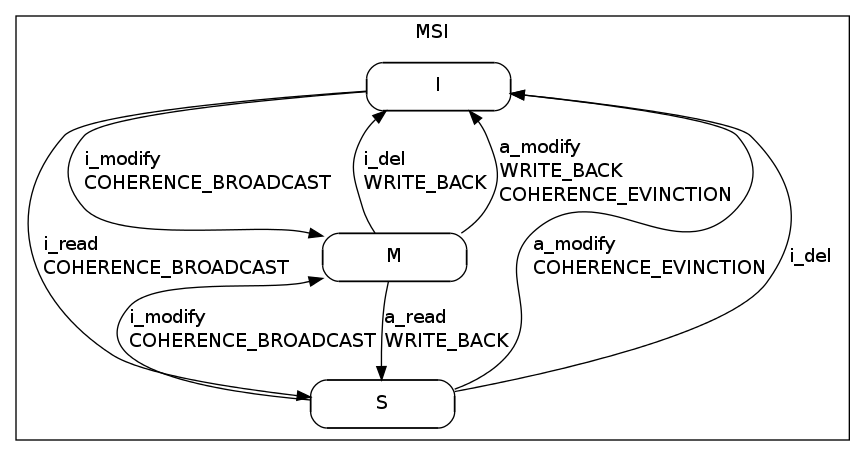
\includegraphics[scale=0.45]{images/MSI_simple.png}
   \caption{\label{img:state_msi} Automate des états MSI}
\end{center}
\end{figure}


\begin{figure}[!h]
\begin{center}
   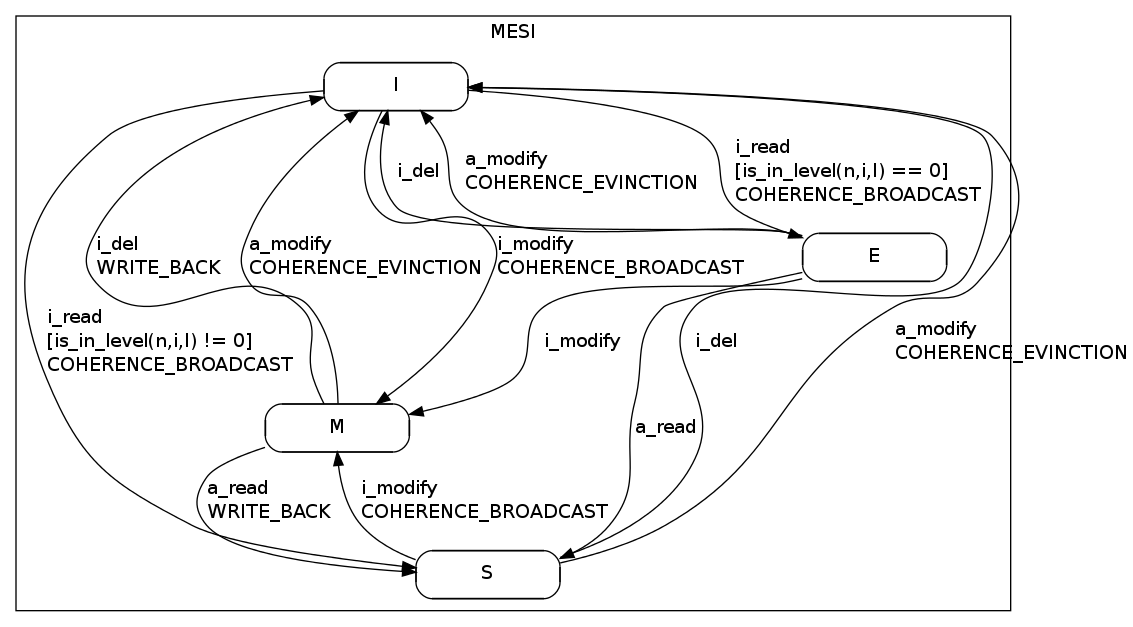
\includegraphics[scale=0.4]{images/MESI_simple.png}
   \caption{\label{img:state_mesi} Automate des états MESI}
\end{center}
\end{figure}


\begin{figure}[!h]
\begin{center}
   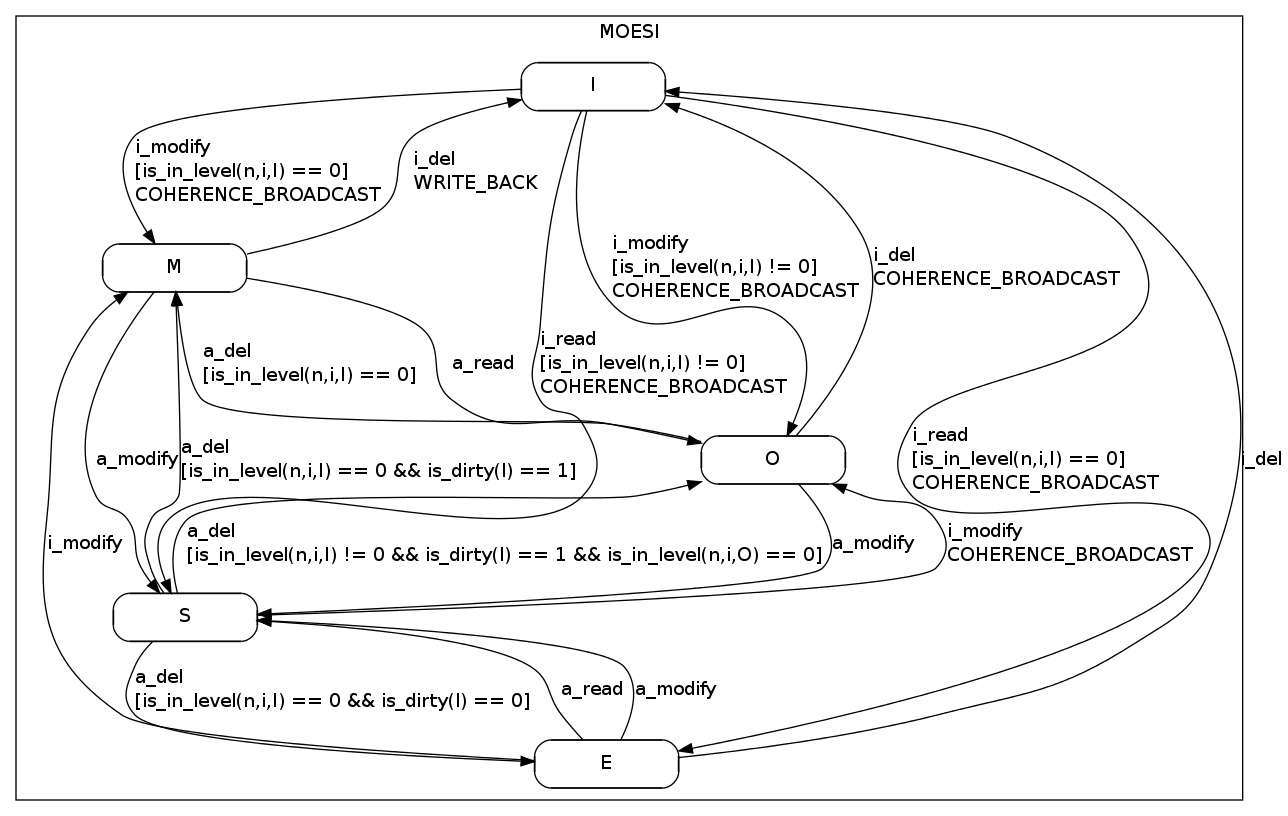
\includegraphics[scale=0.35]{images/MOESI_simple.png}
   \caption{\label{img:state_moesi} Automate des états MOESI}
\end{center}
\end{figure}


\begin{figure}[!h]
\begin{center}
   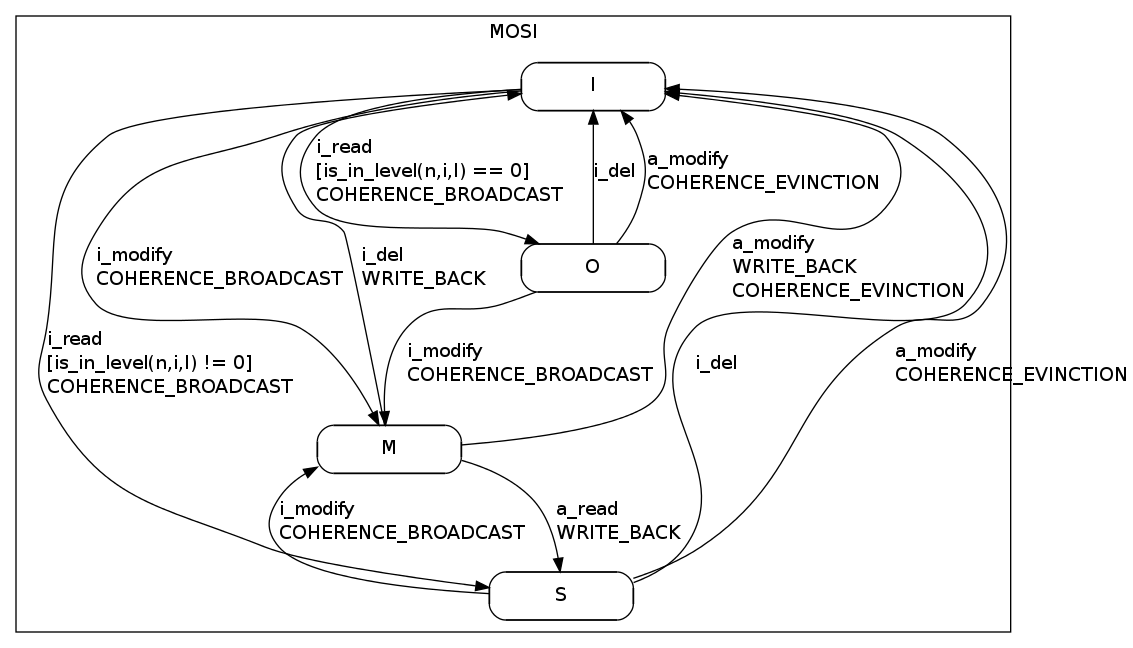
\includegraphics[scale=0.4]{images/MOSI_simple.png}
   \caption{\label{img:state_mosi} Automate des états MOSI}
\end{center}
\end{figure}


\begin{figure}[!h]
\begin{center}
   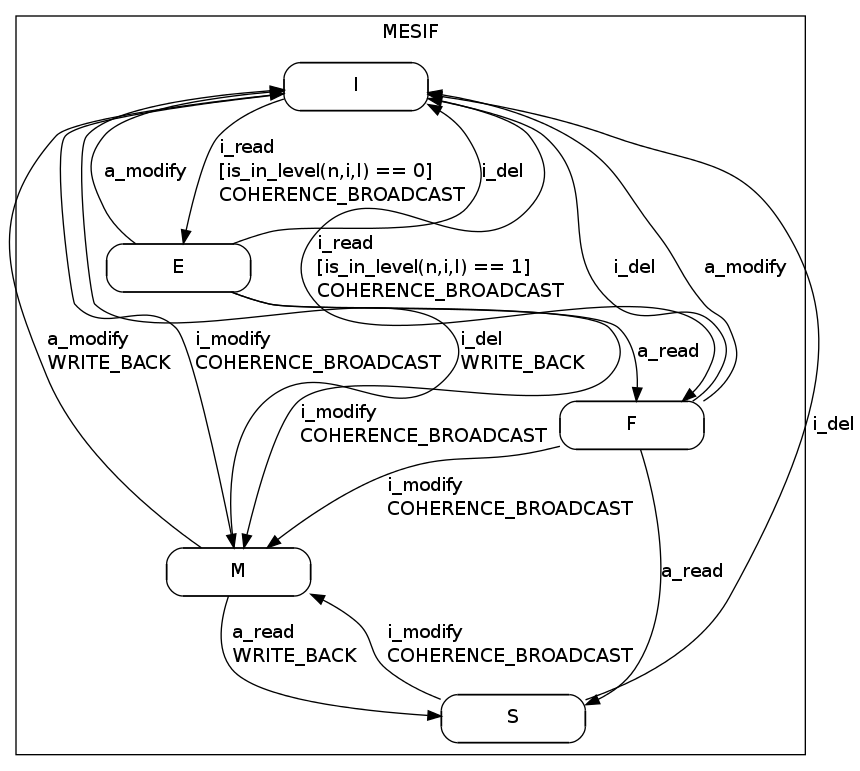
\includegraphics[scale=0.5]{images/MESIF_simple.png}
   \caption{\label{img:state_mesif} Automate des états MESIF}
\end{center}
\end{figure}



\chapter{Tutoriel d'ajout d'une politique de cohérence/remplacement}
\section{Ajout d'une politique de remplacement}

\paragraph{}
Les politiques de remplacement mises en {\oe}uvre dans \textsf{Cassis} sont assez classiques. Il est envisageable d'en rajouter, qui par exemple utiliseraient plus de statistiques en interne pour mieux choisir les données à évincer.

\paragraph{}
Grâce à l'utilisation de pointeurs de fonctions, l'appel de la politique de remplacement voulue au sein d'un cache se fait de façon automatique dans la partie du code qui effectue les actions à réaliser en cas de \emph{load} ou \emph{store}. Il faut ajouter trois fonctions au total :
\begin{itemize}
\item \texttt{(void) replacement\_POLICY(cache)}, dans \texttt{cache.c}
\item \texttt{(void) update\_lines\_POLICY(block, nb\_ways, entry)}, dans \texttt{block.c}
\item \texttt{(int) id\_line\_to\_replace\_POLICY(block, priorité, not\_rm)}, dans \texttt{block.c}
\end{itemize}

\paragraph{}
La première fonction sert à initialiser la structure contenant les pointeurs de fonctions sur les deux fonctions suivantes. Cependant il faut que l'architecture puisse appeler la bonne fonction d'initialisation. Pour cela, il suffir de rajouter, dans la fonction get\_replacement\_fun\-ction(cache), présente dans \texttt{architecture.c}, une entrée vers la nouvelle politique.

\paragraph{}
La seconde sert à mettre à jour les flags de remplacement relatifs à la nouvelle politique, alors que la troisième sert à identifier la ligne à supprimer lorsqu'un cache est plein. A noter que les paramètres priorité et not\_rm servent à améliorer le fonctionnement global des politiques de cohérence. La priorité est utilisée dans le cas de l'usage de \emph{directory manager} pour identifier les données qui sont présentes dans les caches en dessous alors que le paramètre not\_rm sert à identifier une donnée qui va très probablement être ajoutée dans un futur proche. Ces deux paramètres sont toutefois facultatifs, ils n'empêchent pas de fournir des résultats cohérents, et leur utilisation peut être inutile pour une nouvelle politique.

\paragraph{}
La politique de remplacement peut se baser sur toutes les données stockées dans les structures \texttt{block} et \texttt{line}. Actuellement c'est l'entier \texttt{line.use} qui est utilisée, mais l'utilisateur peut ici décider d'en rajouter, ou de se baser sur d'autres informations telles que l'état de la ligne.

\paragraph{}
Pour ajouter une politique de remplacement plus globale permettant par exemple d'obtenir des informations à partir d'autres caches, il faut modifier le prototype de fonction pour prendre un n{\oe}ud à la place d'un bloc. Il faudra cependant s'assurer de modifier toutes les fonctions existantes pour les trois politiques déjà implémentées.

\section{Ajout d'une politique de cohérence}
\label{tuto_aut}

\subsection{Sources à modifier}

Les politiques de cohérence sont toutes décrites dans un seul fichier, écrit grâce à \textsf{SMC} : \texttt{coherence.sm}. Toutefois d'autres sources sont à modifier afin que ces politiques puissent être choisies depuis un fichier d'architecture.

\subsubsection{\texttt{common\_types.h}}

Il faut modifier dans ce fichier les deux énumérations \texttt{status} et \texttt{cache\_coherence} qui contiennent pour la première les status possibles pour les lignes, et pour la seconde les noms des politiques de cohérence.

\subsubsection{\texttt{architecture.c}}

L'analyse du fichier d'architecture en \texttt{XML} doit reférencer le nom de la nouvelle politique POLICY. Pour cela il faut rajouter le cas adéquat dans la fonction \texttt{coherence(...)} de ce fichier.

\subsubsection{\texttt{coherence.c}}

La fonction \texttt{coherence\_init(...)} initialise l'automate vers la bonne politique de cohérence. Il convient ici d'appeler la transition qui permet de passer de la carte\footnote{Notons que nous parlons ici de \og carte \fg. En effet il n'y a qu'un seul automate contenant toutes les politiques du point de vue de \textsf{SMC}, mais pouvant s'appuyer sur plusieurs cartes. Chacune des cartes correspond à la vision classique d'un automate de cohérence, nous continuerons ici d'employer le terme \og carte \fg afin de distinguer l'automate tel que vu par \textsf{SMC} (qui correspond à l'ensemble des politiques, plus l'initialisation), de l'automate de cohérence d'une politique, appelé ici \og carte \fg.} de l'automate de départ vers la carte de l'automate POLICY. Le cas à rajouter ne peut être ici fait que d'une seule façon, avec un nom précis de fonction :
\begin{framed}
\begin{lstlisting}[frame=none,language=C]
  case POLICY:
    coherenceContext_POLICY(&this->_fsm);
    break;
\end{lstlisting}
\end{framed}
Cela nécessite de nommer la carte de cette politique de cohérence POLICY dans le point suivant.

\subsubsection{\texttt{coherence.sm}}


Deux parties sont à modifier dans ce fichier. La première permet de changer de carte vers la bonne politique :
\begin{framed}
\begin{verbatim}
%map Init
%%
// State    Transition  End State       Action(s)
Start
{
            MSI        jump(MSI::I)     {}
            ...
            ...
            POLICY     jump(POLICY::I)  {}
}
%%
\end{verbatim}
\end{framed}

Par ailleurs il faut rajouter après cette première carte, la carte de la nouvelle politique, il s'agit ici d'une recopie de MSI :
\begin{framed}
\begin{verbatim}
%map POLICY
%%
// State         Transition        End State       Action(s)

I
{
	i_modify(n: struct node*, i: unsigned long, l: struct line*)       
            M      {modify_line(l); up_stat(n,i,COHERENCE_BROADCAST);}
	i_read(n: struct node*, i: unsigned long, l: struct line*)         
            S      {share_line(l); up_stat(n,i,COHERENCE_BROADCAST);}           
}

M
{
	a_read(n: struct node*, i: unsigned long, l: struct line*)        
            S       {share_line(l);up_stat(n,i,WRITE_BACK);
                     dirty_line(l, 0);}
	i_del(n: struct node*, i: unsigned long, l: struct line*)         
            I       {invalid_line(l);up_stat(n,i,WRITE_BACK);}     
	a_modify(n: struct node*, i: unsigned long, l: struct line*)      
            I       {invalid_line(l);up_stat(n,i,WRITE_BACK);
                     up_stat(n,i,COHERENCE_EVINCTION);}
}

S
{
	i_modify(n: struct node*, i: unsigned long, l: struct line*)      
            M       {modify_line(l);up_stat(n,i,COHERENCE_BROADCAST);}
	a_modify(n: struct node*, i: unsigned long, l: struct line*)      
            I       {invalid_line(l);up_stat(n,i,COHERENCE_EVINCTION);}
	i_del(n: struct node*, i: unsigned long, l: struct line*)         
            I       {invalid_line(l);}                 
}


Default
{
	i_read(n: struct node*, i: unsigned long, l: struct line*)     nil    {}
	i_modify(n: struct node*, i: unsigned long, l: struct line*)   nil    {}
	i_del(n: struct node*, i: unsigned long, l: struct line*)      nil     {}
	a_read(n: struct node*, i: unsigned long, l: struct line*)     nil    {}
	a_modify(n: struct node*, i: unsigned long, l: struct line*)   nil    {}
	a_del(n: struct node*, i: unsigned long, l: struct line*)      nil     {}

}
%%
\end{verbatim}
\end{framed}

Remarquons que l'état \verb!Default! permet ici de créer une boucle sur tous les états ne définissant pas toutes les transitions possibles. Cela évite de définir les transitions qui ne donnent pas lieu à un changement d'état ni à des actions particulières. Il est par ailleurs nécessaire que \verb!Default! soit présent, soit toutes les transitions soient définies pour chaque état, car l'automate ne fonctionnera pas si une transition est appelée sur un état qui ne la définit pas.


\subsection{Actions possibles}

L'exemple de code précédent contient déjà quelques unes des possibilités offertes par \textsf{SMC}. Toutefois, il y a d'une part d'autres possibilités -- notamment les transitions conditionnelles -- et d'autre part quelques restrictions. L'usage de \textsf{SMC} n'est pas vu en détail ici, pour cela il est possible de consulter la documentation officielle sur leur \href{http://smc.sourceforge.net/SmcManual.htm}{site}. Seuls quelques aspects sont ici précisés, et notamment les liens avec les fichiers du simulateur.

\paragraph{Arguments des transitions.}
Les arguments des transition peuvent utiliser n'importe quel type primaire de \texttt{C}, mais en ce qui concerne les structures, il faut alors qu'elles soient redéclarées au tout début du fichier, mais si celles-ci sont présentes dans les inclusions du fichier \texttt{coherence.h}.
\begin{framed}
\begin{verbatim}
%declare struct node;
%declare struct line;

%start Init::Start
%class coherence
%header coherence.h
\end{verbatim}
\end{framed}

\paragraph{Transitions conditionnelles.}
Il est possible de définir plusieurs fois la même transition avec des conditions différentes, afin de permettre de passer dans un autre état, ou bien de faire d'autres actions que la première définition. Les conditions sont des comparaisons simples écrites en \texttt{C}. Par exemple :
\begin{framed}
\begin{verbatim}
a_del(n: struct node*, i: unsigned long, l: struct line*)  
    [is_in_level(n,i,I) != 0 && is_dirty(l) == 1 
                             && is_in_level(n,i,O) == 0] 
          O       {owned_line(l);}

a_del(n: struct node*, i: unsigned long, l: struct line*)    
    [is_in_level(n,i,I) == 0 && is_dirty(l) == 1]   
          M       {modify_line(l);}
\end{verbatim}
\end{framed}
Les fonctions appelées par les conditions doivent être définies depuis les inclusions du fichier \texttt{coherence.h}.

\paragraph{Code dans les actions.}
Le code dans les actions ne peut \emph{a priori} qu'être une succession d'appels de fonctions avec une règle de nommage spécifique. En effet toute fonction appelée depuis les règles d'actions dans le fichier \texttt{coherence.sm} doit être définie (dans une des inclusions comme précédemment) avec le même nom préfixé par \texttt{coherence\_}. En effet \textsf{SMC} était à l'origine prévu pour des langages orientés objet, et pour le \texttt{C} il est tout de même nécessaire de préciser une classe, ici \texttt{coherence}. Pour plus de précisions sur les actions à effectuer, voir la section \ref{actions}.

\paragraph{Ajout de transition.}
L'ajout d'une transition nécessite beaucoup de modifications. D'une part il faut l'ajouter dans toutes les cartes pour garder l'indépendance de l'appel de la cohérence vis-à-vis des différentes politiques possibles. D'autre part \textsf{SMC} introduit ici encore une obligation syntaxique, la définition de la transition dans \texttt{coherence.sm} et la fonction telle que définie par le \texttt{coherence\_sm.h } n'ont en effet pas les mêmes prototypes :
\begin{framed}
\begin{verbatim}
\\dans coherence.sm :
i_del(n: struct node*, i: unsigned long, l: struct line*)
\\tel qu'appelé depuis add_line_hierarchy.c :
coherenceContext_i_del(&line->coher->_fsm, current_node, entry, line);
\end{verbatim}
\end{framed}

\nocite{*}
\bibliographystyle{plain}
\bibliography{rapport}

\end{document}
